\chapter{Parameter Distributions and Detection Probabilities}\label{ch:param_dists}

\section{Current State of Knowledge}\label{sec:curr_param_dists}
The distributions of the physical and orbital parameters of exoplanets change rapidly as the pace of exoplanet discovery accelerates.  As of this writing, this entire population is being transformed as the Kepler mission continuously introduces new candidates potentially doubling the total number of known exoplanets \citep{borucki2010kepler}.  Multiple groups are maintaining and updating catalogues of exoplanets and are actively working on deriving the distributions of planetary and orbital parameters \citep{marcy2005observed,cumming2008,mordasini2009extrasolarI,mordasini2009extrasolarII}.  One of the most important results of this work is the identification of a power-law trend in the relationship between projected mass ($m_P \sin I$) and period in radial velocity survey data.  \reffig{fig:cummingData} shows data from the Keck planet search, while \reffig{fig:cummingMPfit} shows the resulting power-law fit to the model:
\begin{equation}\label{eq:powerlawModel}
\intd{N}  =  c m_P^\alpha P_{orb}^\beta \intd{\log m_P}  \intd{\log P_{orb}} \,,
\end{equation}
where $c$ is a constant of proportionality.  This work is very useful in generating sample planetary systems as in \S\ref{sec:gen_plan_sys}.

\begin{figure}[ht!]
\centering
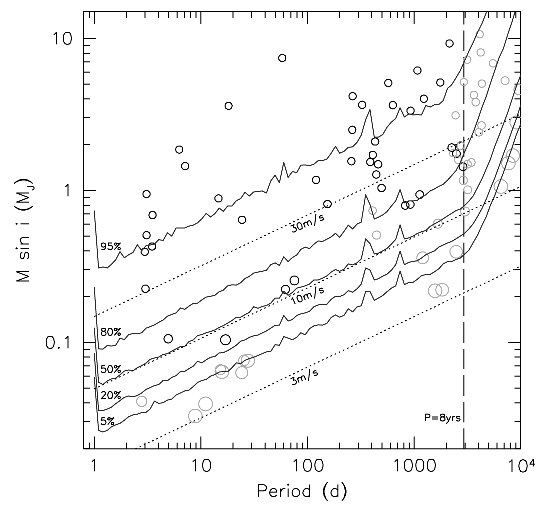
\includegraphics[width=5.5in]{./figures/cummingData}
 \caption[$m_P\sin I - P_{orb}$ Data]{ Detections for F, G, and K stars corrected for completeness of the survey. Black circles are confirmed planets circa May 2005 and gray circles are candidates with circle size indicating the magnitude of selection effects for each. The vertical dashed line indicates a period of 8 years and the dotted lines show velocity amplitudes of 3, 10, and 30 m/s for a 1 M$_\odot$ star. For a given period, the solid curves show the mass that can be ruled out at the 99\% level from 5\%, 20\%, 50\%, 80\%, and 95\% of stars. From \citet{cumming2008}.}
\label{fig:cummingData} 
\end{figure} 

\begin{figure}[ht]
\centering
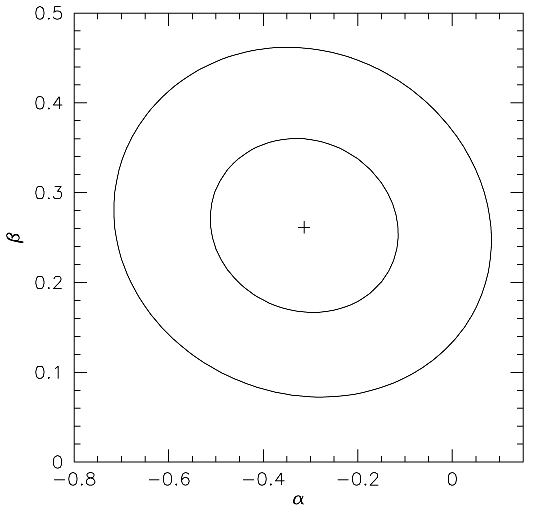
\includegraphics[width=4.5in]{./figures/cummingMPfit}
 \caption[$m_P\sin I - P_{orb}$ power-law fits]{ Contours of constant likelihood for a fit to \refeq{eq:powerlawModel} . The contours correspond to the 68\% and 95\% confidence intervals with best-fit values of  $\alpha = -0.31$ and $\beta = 0.26$.  From \citet{cumming2008}.}
\label{fig:cummingMPfit} 
\end{figure} 

Similarly, much work has been done to constrain the density distributions of known planets, relating planetary masses and radii.  As shown in \citet{fortney2007}, the densities of rocky planets can be modeled to a high degree of accuracy by assuming that the planets are composed of either a rock/ice or a rock/iron mixture.  These assumptions lead to the relations:
\begin{equation}\label{eq:rockyPlanDensities}
R = \left\{ \begin{array}{l l} 
\begin{array}{l} (0.0912(1-\textrm{rmf}) + 0.1603)(\log m_P)^2\\ + (0.3330(1-\textrm{rmf}) + 0.7387)\log m_P \\
{} + (0.4639 (1-\textrm{rmf}) + 1.1193) \end{array} & \textrm{ice/rock} \\\\
\begin{array}{l} (0.0592\textrm{rmf} + 0.0975)(\log m_P)^2\\ + (0.2337\textrm{rmf} + 0.4938)\log m_P \\
{} + (0.3102\textrm{rmf} + 0.7932) \end{array} & \textrm{rock/iron}
\end{array} \right.
\end{equation}
where the planetary radius is measured in $R_\oplus$, the planetary mass in $M_\oplus$ and rmf is the fraction of rock.  The resulting density curves are shown in \reffig{fig:fortneyDensities}.  For giant planets, radii values may be interpolated from a lookup table based on known values by assuming the fraction of the planet's mass contained in the core \citep{fortney2007}.  Density modeling is especially important in simulating direct imaging as both the planet radius and planet mass must be defined to generate the observable quantities and to propagate the planet on its orbit.

\begin{figure}[ht]
\centering
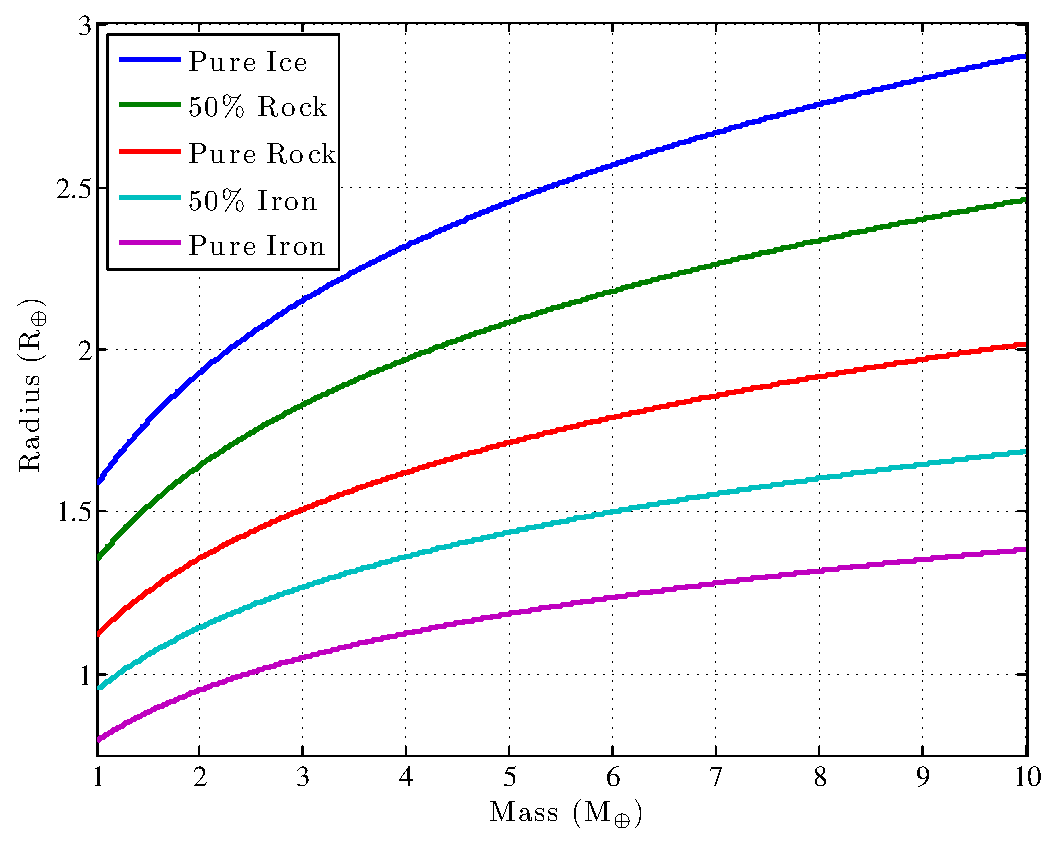
\includegraphics[width=5.5in]{./figures/fortneyDensities}
 \caption[Rocky planet densities]{ Densities of rocky planets modeled as rock/ice and rock/iron mixtures \citep{fortney2007}.}
\label{fig:fortneyDensities} 
\end{figure} 

Another important observed correlation is between the occurrence of exoplanets and the metallicity of the host star.  Surveying a population of  FGK stars, \citet{marcy2005observed} found planets around approximately 25\% of the most metal-rich stars (i.e.,  [Fe/H] > 0.3) and around only 3\% of metal poor stars ([Fe/H] < -0.5).  The occurence of planets as a function of [Fe/H] can also be fit to a power-law---gas giant detections are nearly proportional to the square of the number of iron atoms of the host star, with constant of proportionality of about 0.03 (\reffig{fig:marcyFEH}).  This may be an important factor in the selection of a target list, especially as a final filter to pinpoint the highest detection probability targets (see \S\ref{sec:targ_selection}).

\begin{figure}[ht]
\centering
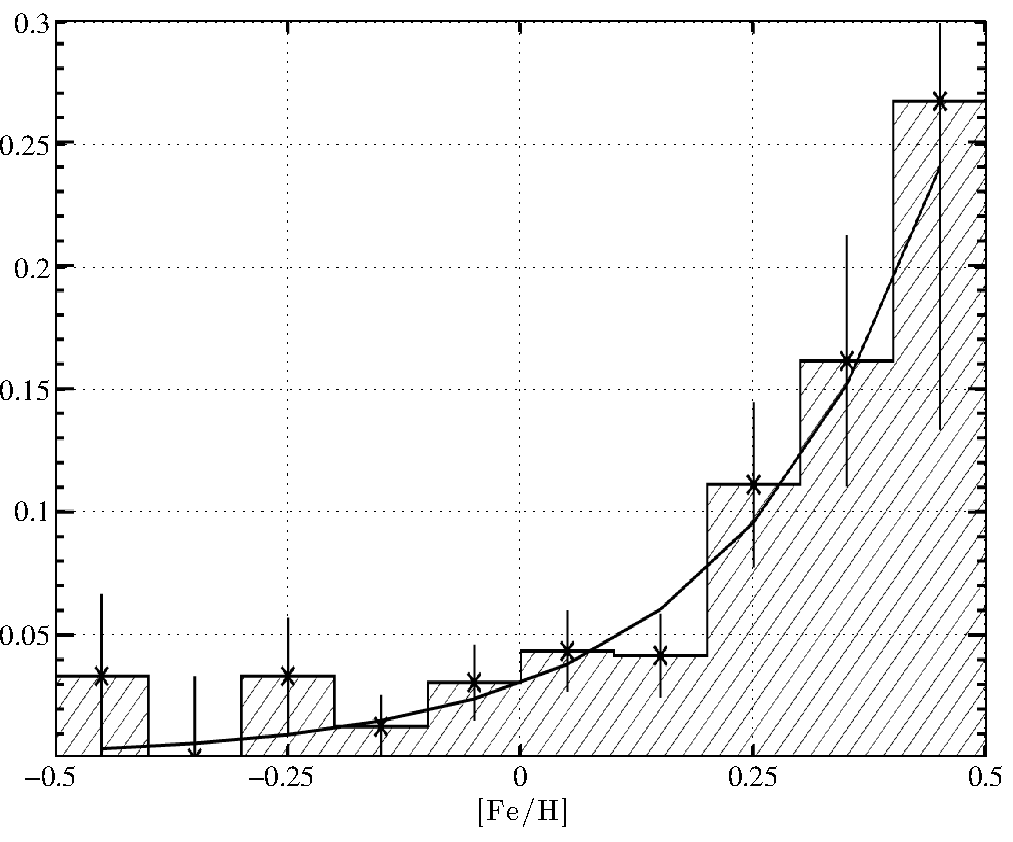
\includegraphics[width=5.5in]{./figures/marcyFEH}
 \caption[Planet occurence vs metallicity]{ Portion of host stars with planets as function of iron abundance [Fe/H] star. Data from \citet{marcy2005observed}.}
\label{fig:marcyFEH} 
\end{figure} 


\subsection{Biases}\label{sec:biases}
If we plot a snapshot of the available orbital parameters for the currently known exoplanets, as in \reffig{fig:currHists}, we immediately notice several prominent, and potentially misleading, features.  There appears to be a large bias towards low eccentricity and semi-major axis.   The low semi-major axes preference is due to the inherent bias in detection methods that require full (or even multiple) periods of data before a detection can be validated.  These methods inherently detect more short period planets and as they include astrometry, radial velocity and transit photometry, which were used to find the majority of known exoplanets, the data set contains a disproportionately large number of short period (and thus low semi-major axis) planets.  The low eccentricity accumulation is due to a specific population of planets: tidally locked short period gas giants  or `hot Jupiters'.  These are easily detected due to their large size and short period, and all have near zero eccentricity due to orbital circularization.

\begin{figure}[ht]
\centering
\subfigure[Mass]{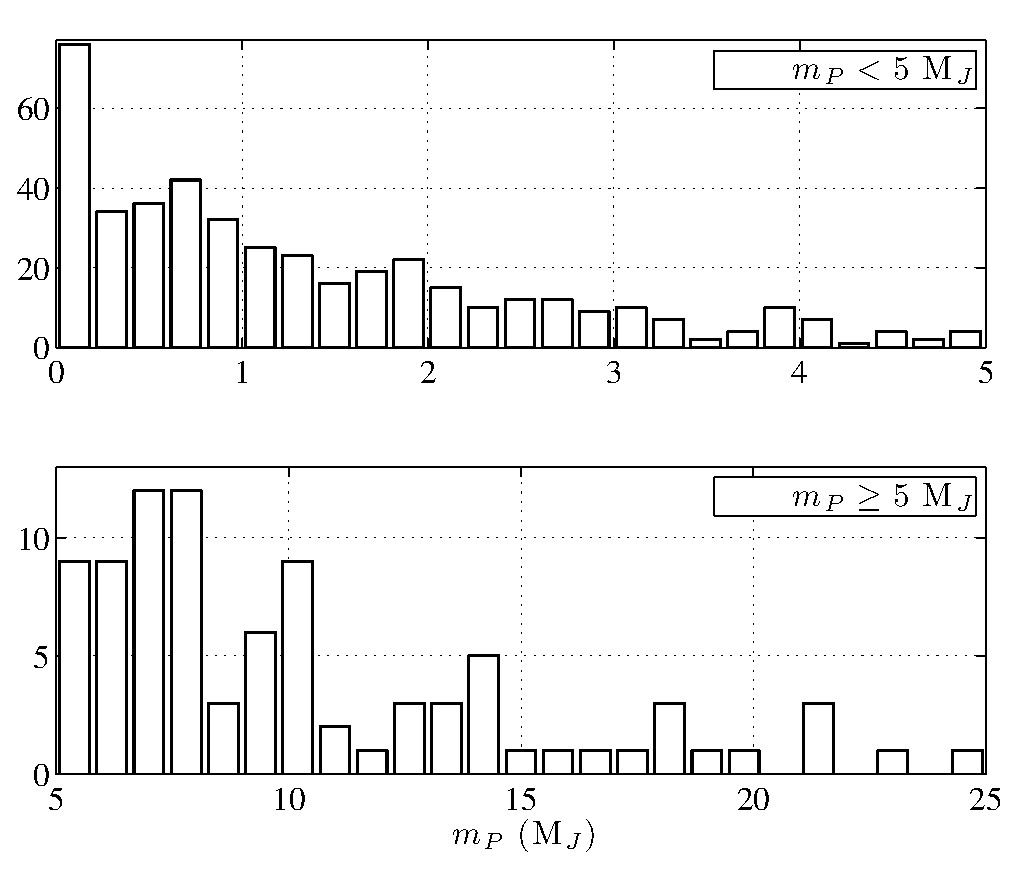
\includegraphics[width=2.9in]{./figures/currMassHist}\label{fig:currMassHist}}
\subfigure[Semi-major axis]{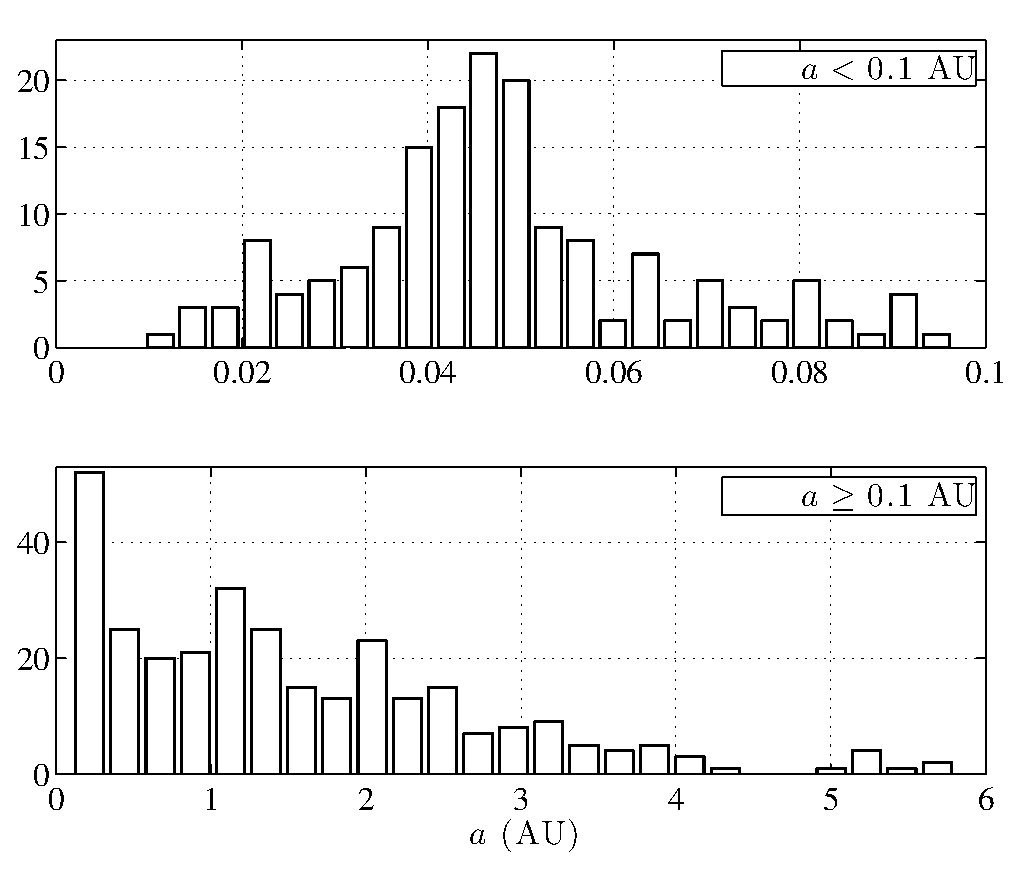
\includegraphics[width=2.9in]{./figures/currSMaxHist}\label{fig:currSMaxHist}}
\subfigure[Eccentricity]{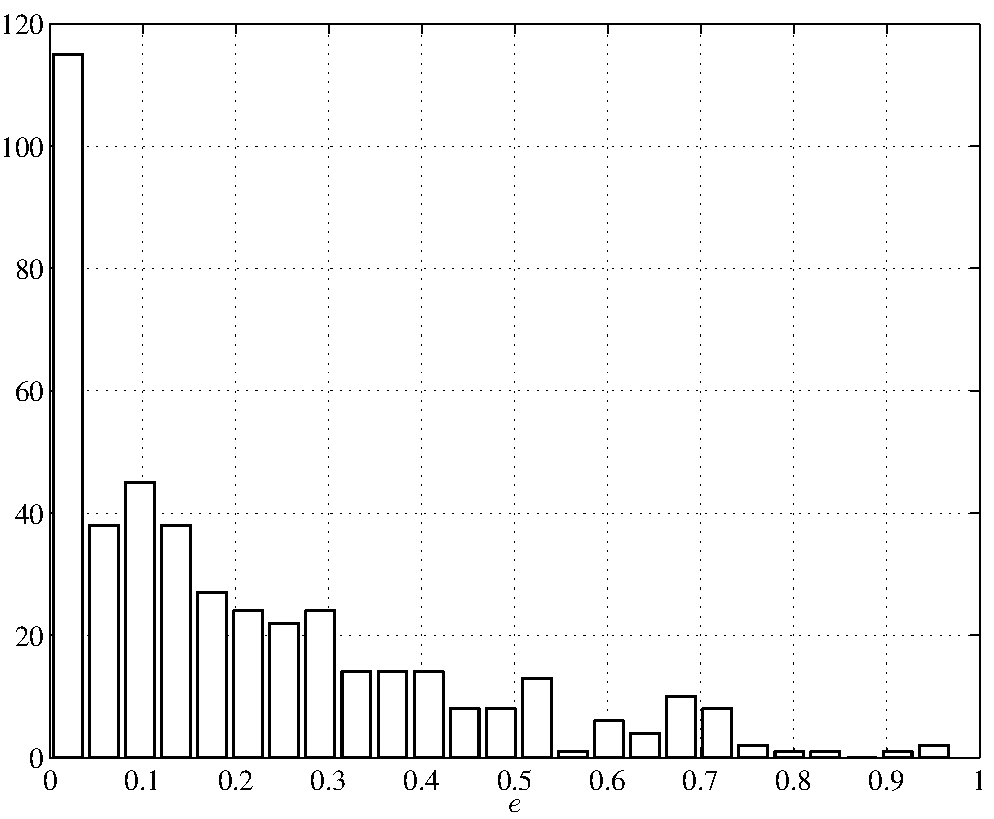
\includegraphics[width=3.5in]{./figures/currEccenHist}\label{fig:currEccenHist}}
 \caption[Orbital parameter distributions of currently known exoplanets]{Histograms of orbital parameters of currently known exoplanets. Retrieved from the NASA/IPAC/NExScI Star and Exoplanet Database \url{http://nsted.ipac.caltech.edu} on April 17th, 2011. \label{fig:currHists}}
\end{figure}  

Much work has been devoted to trying to find the true distributions of these parameters using both detailed modeling \citep{currie2009semimajor} and data analysis \citep{hogg2010inferring}.  These efforts all seek to incorporate not just the raw data, but also the instrumental biases and the likelihoods of the individual detections.  Another important point is to consider inherent biases in the parameters themselves---for example, as eccentricity is defined within a strictly bounded range, it tends to be overestimated, introducing another source of bias.  In the remainder of this chapter, we will consider how to model the likelihood of planetary detections, as well as the Keplerian elements used for describing planetary orbits.

\section{Observational Completeness}\label{sec:completeness}
\citet{brown2004a} introduced the concept of completeness to study the selection effects introduced by observatory architectures on direct detection searches for sub-stellar companions.  Assuming distributions for the semi-major axis and eccentricity of planetary orbits, Brown calculated the probability that a companion's angular separation would fall outside the telescope's IWA during an observation of its parent star.  \citet{brown2005} subsequently expanded this concept to include the selection effects due to the telescope specific photometric restrictions on observability (i.e., $\Delta$mag$_0$), and \citet{brown2009} demonstrated how completeness could be evaluated for indirect companion detection methods such as astrometry.  Completeness has also been extended to account for multiple observations of one star at different times \citep{brown2010new}, and has been utilized in mission analysis and development for a variety of proposed exoplanet observatories \citep{savransky2010,brown2009} as will be detailed in \refch{ch:obs_sims}.

The direct detection completeness is evaluated by assuming that a companion will be observable if its angular separation from the star is greater than the observatory's IWA, and illuminated such that the difference in brightness between star and companion is below the limiting $\Delta$mag.  To calculate the completeness, probability distributions (or constant values) are assumed for planetary orbital elements and physical properties.  A large, equal number of samples is generated from each distribution, and the star-planet angular separation and $\Delta$mag are calculated for each set of samples.  When binned in a two-dimensional histogram, these generate a density function representing the probability that a planet drawn at random from the assumed population will have a given angular separation and $\Delta$mag (\reffig{fig:earthTwin_pdf}).  Integrating over this density yields a cumulative distribution function (CDF).  An instrument with a given $\Delta$mag$_0$ and IWA, observing a star with a planet from the assumed population, has a probability of detecting the planet upon its first observation equal to the corresponding CDF point \reffig{fig:earthTwin_cdf}).

\begin{figure}[ht]
\centering
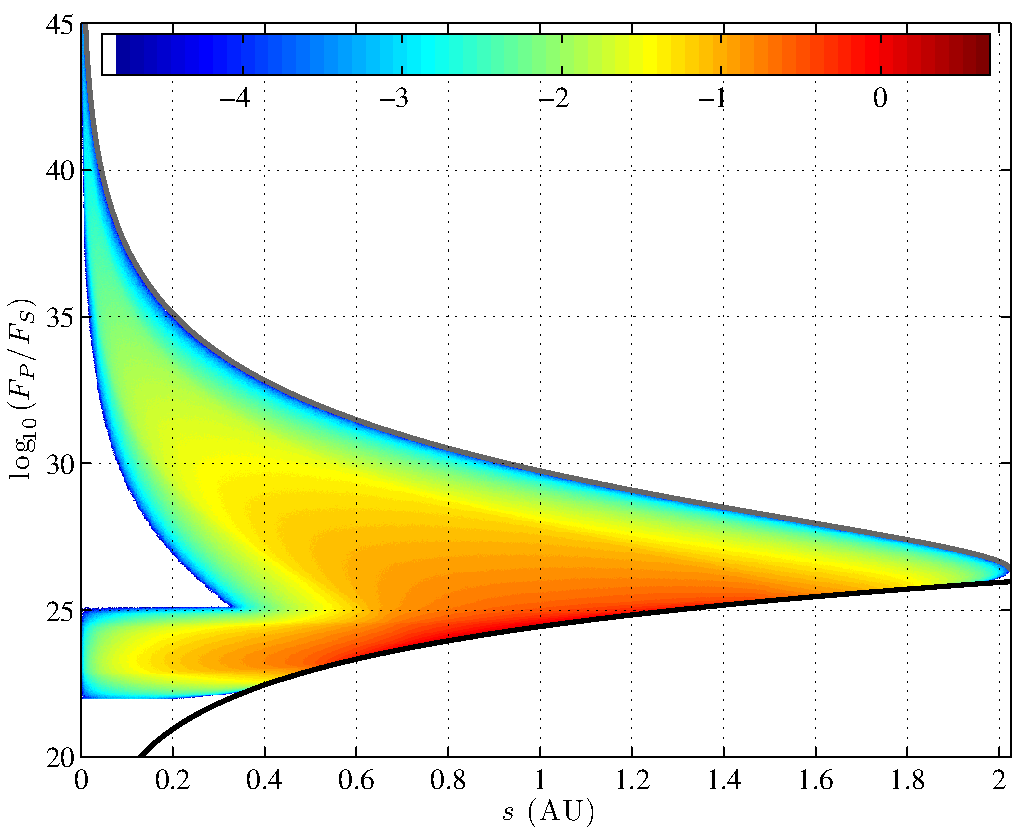
\includegraphics[width=5.5in]{./figures/earthTwin_pdf}
 \caption[Earth-twin observation PDF]{ Observational and photometric completeness for a population of Earth-twin planets ($a \in [0.7, 1.5]$, $e \in [0, 0.35]$, $p = p_\oplus$, $R = R_\oplus$).  The joint probability density function of ($\bar s = s,\bar F_P/F_S = F_P/F_S$) is sampled via 1 billion Monte Carlo trials, and the 2D histogram is constructed by counting the number of occurrences in each grid square scaled by total number of samples and the grid square area. The colorbar is log-scale, in powers of 10 and the bounding solid lines (black and gray) are calculated via Equations (\ref{eq:maxFr}) and (\ref{eq:minFr}).  The black line does not bound the histogram for all values of $s$ because of the limits on $a$ placed on the input distribution.}
\label{fig:earthTwin_pdf} 
\end{figure} 

\begin{figure}[ht]
\centering
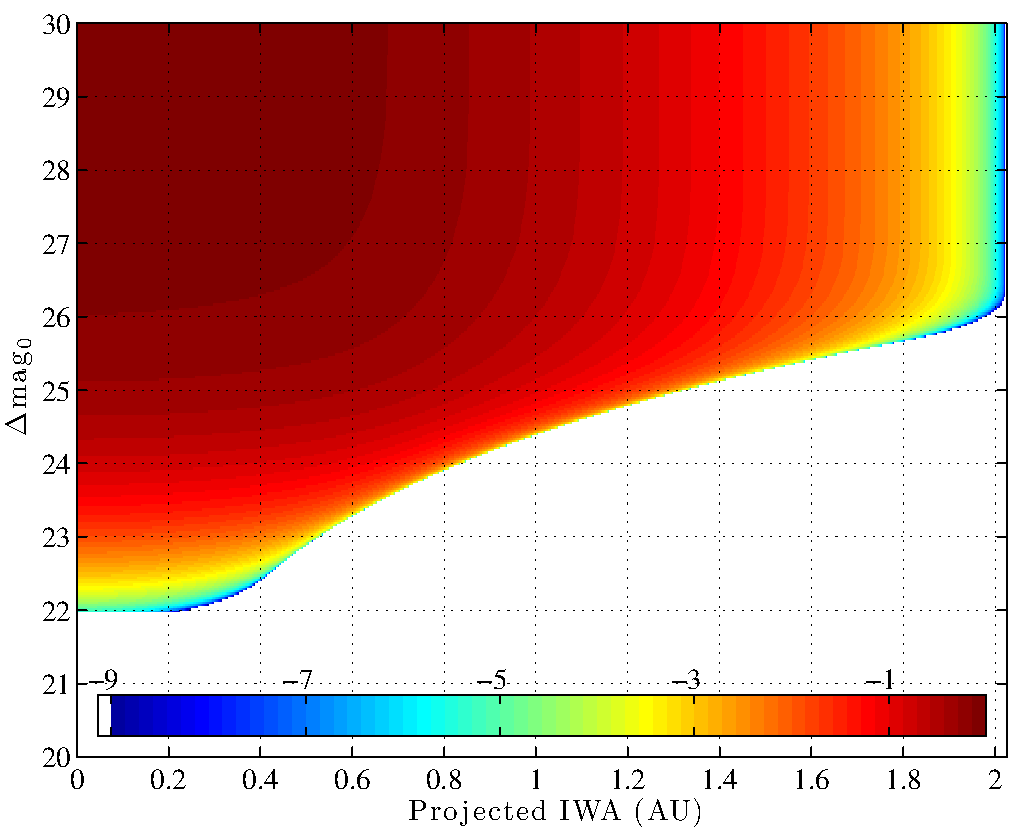
\includegraphics[width=5.5in]{./figures/earthTwin_cdf}
 \caption[Earth-twin observation CDF]{Integrated observational and photometric completeness from \reffig{fig:earthTwin_pdf}. The colorbar is log-scale, in powers of 10, representing the cumulative distribution function of the random variable in \reffig{fig:earthTwin_pdf}.  The CDF is calculated by summing across the rows and columns of the (unscaled) PDF histogram at each grid square and scaling the result by the total number of samples.  The histogram is truncated at $\Delta$mag$_0$ of 30, as the CDF becomes nearly constant for a given projected IWA for $\Delta$mag$_0 > 27$, as demonstrated by the vertical bands of nearly constant color.  The CDF is unity at zero projected IWA and $\Delta$mag$_0 > 53$.}
\label{fig:earthTwin_cdf} 
\end{figure} 

\subsection{Applications}\label{sec:completeness_apps}
This definition of completeness describes the conditional detection probability (given the instrument capabilities and that a planet exists in the target system) only for the first target system observation.  Subsequent observations of the same exosystem do not represent independent samples, and will thus have different detection probabilities.  If each observation was fully independent of the others, with constant detection probability ($p_c$) equal to the single visit completeness, then the probability of $k$ successful detections in $n$ visits would be  given simply by the binomial theorem as:
\begin{equation}
P_n(k) = \binom{n}{k} p_c^k (1-p_c)^{n-k} \, .
\end{equation}
The probability of any (non-zero) number of detections in $n$ visits would then be
\begin{equation} \label{eq:multvisit_detprob}
P_n(k>0) = 1 -  \binom{n}{0}  p_c^0 (1-p_c)^{n} = 1 - (1-p_c)^n\, .
\end{equation}
In reality the probability of detecting a planet on subsequent visits is conditionally dependent on the planet's orbit and the times between observations, but this equation gives a good upper bound for the probability of detecting a planet (given that one exists) over multiple visits.  

We can demonstrate this bound empirically by running Monte Carlo simulations of 1 million orbits in the habitable zone of a given star and tracking the aggregate number of detections over multiple visits.  The results are shown in \reffig{fig:compSim}.  All of the planets are modeled as Earth-twins, and the instrument is assumed to have a limiting $\Delta$mag of 26.  The star's luminosity and distance and instrument's IWA  are chosen so that the projected IWA corresponds to the inner edge of the habitable zone (i.e., the projected IWA is at 0.70 AU for a star of 1 L$_\odot$).  The single visit completeness of this star for Earth-twins on habitable-zone orbits is approximately 0.5162.  The plots show the results of returning every 1, 2, and 4 weeks, as well as daily revisits, randomly timed revisits, and the values of \refeq{eq:multvisit_detprob}.  We assume that observations are instantaneous and do not add to the interim period between observations.  In all cases, we eventually are able to observe over 99\% of all planets and $P_n(k >0)$ serves as an upper bound to the probability of planets found in $n$ visits.  Its also interesting to note that the randomized revisit interval most closely approximates the curve generated from \refeq{eq:multvisit_detprob}, giving the largest percentage of planets found in the smallest number of visits.  This makes sense because randomization serves to weaken the dependence of subsequent visits on the time interval.  In essence randomizing return times approximates the conceit of viewing a system over and over again `for the first time'.  Of course, this breaks down after the initial few visits, and we again begin to perform more poorly than the bound.

\begin{figure}[ht]
 \begin{center}
 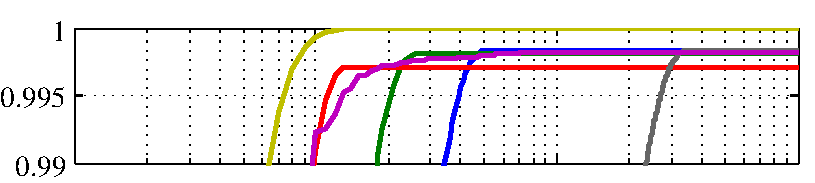
\includegraphics[width=4.34in,clip=true,trim=0in 0in 0.05in 0in]{./figures/compSimZoom}\\
   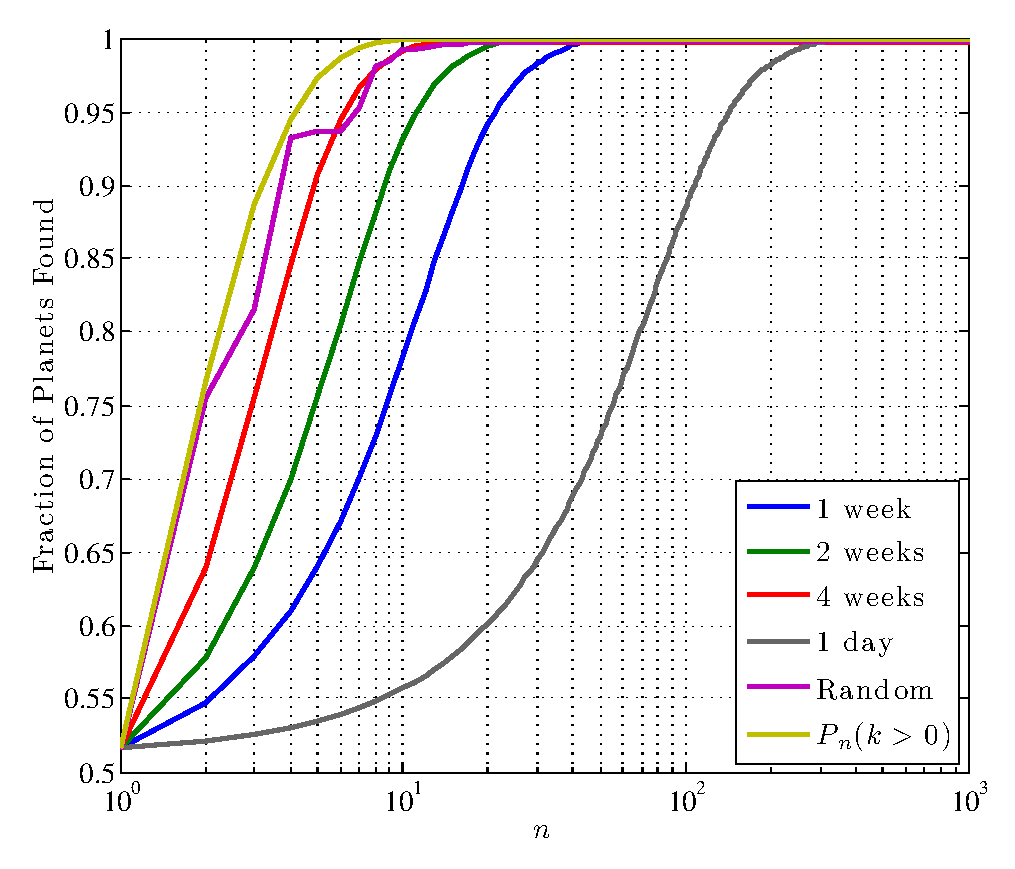
\includegraphics[width=4.5in]{./figures/compSim}
 \end{center}
 \caption[Planet detection probability over multiple visits]{ \label{fig:compSim} 
	The fraction of planets found as a function of number of visits, with various intervals between observations, as well as the bounding probability given by \refeq{eq:multvisit_detprob}.  The curve marked `Random' represents randomized revisit intervals, uniformly distributed within one mean period of the population.  The top panel is a zoomed view of the top 1\% of the plot.}
\end{figure} 

The exception to the bound given by \refeq{eq:multvisit_detprob} would be the case of an optimal observing strategy (i.e., one where we only see previously unobservable portions of the habitable zone on each subsequent visit) on a fully observable system (i.e., one where all parts of the habitable zone are observable at some point).  In the optimal scenario, a new portion of the habitable zone equal to the fraction represented by $p_c$ is observed at each visit and the schedule is such that each portion is observed in sequence so no planets could be bypassed (the equivalent of a continuous observation).  If such an observing schedule could be achieved, the probability of detecting a planet after $1/p_c$ visits would be unity.  For the majority of targets, however, it is quite difficult to follow the strict timing dictated by this strategy.  Because target stars may only be observed for specific intervals of time at given times of the year\footnote{These observable time periods are known as `observing seasons' and are determined by an observatory's keep-out zone, which is discussed in \S\ref{sec:targ_selection}}, it is often impossible to follow the optimal observing schedule in the limited period defined by the mission lifetime.  It is because of these constraints that we often fail to detect existing planets even when the target system has been visited enough times to yield a high probability of detection.  \refeq{eq:multvisit_detprob} always holds as an upper bound for systems with permanently unobservable sections of the habitable zone (where the habitable zone is partially inside the projected IWA).

In the case of only one visit per target star, the calculation of overall detection probability is actually much simpler, and equals the sum of the targets' single visit completeness values.  If all of the targets have the same completeness (fixed $p_c$), then the expected number of planets found ($Y$), given that each star has one ($\eta_\oplus = 1$), is:
\begin{equation}
E[Y] = \sum_{k = 1}^n k \binom{n}{k}  p_c^k (1-p_c)^{n-k} = np_c \,.
\end{equation}
Because $Y$ is the sum of $n$ Bernoulli random variables, each of which has expected value $p_c$, the expected value of $Y$ must be $np_c$.  If the target stars all have different single visit completeness values (non-constant $p_c$), the expected value of $Y$ for $n$ targets with completeness values of $\{p_i\}_{i=1}^n$ is:
\begin{equation}
E[Y] = \sum_{k = 1}^n k  \sum_{j \in \leftsub{n}{C}_k} \prod_{i \in j} p_i  \prod_{i \notin j} (1 - p_i) = \sum_{i = 1}^n{p_i}  \,,
\end{equation}
where $ \leftsub{n}{C}_k$ is the set of combinations of the values from 1 to $n$ taken $k$ at a time.

\section{Analytical Distributions}\label{sec:analytic_dists}
The procedure described in the previous section for generating the completeness function is a Monte Carlo sampling of a bivariate distribution function of non-independent arguments (since star-planet separation and $\Delta$mag are functions of the same parameters).  Thus in order to find any one point (or section) of the completeness distribution, it is necessary to sample it completely.  Because of the relatively high dimensionality of the initial parameter space and wide range of values certain parameters can take, complete sampling requires a large number of Monte Carlo trials.  For example, even with 100 million samples certain low probability areas of the function are significantly under-sampled, as demonstrated in \reffig{fig:undersampled_comp_pdf}.

\begin{figure}[ht]
\centering
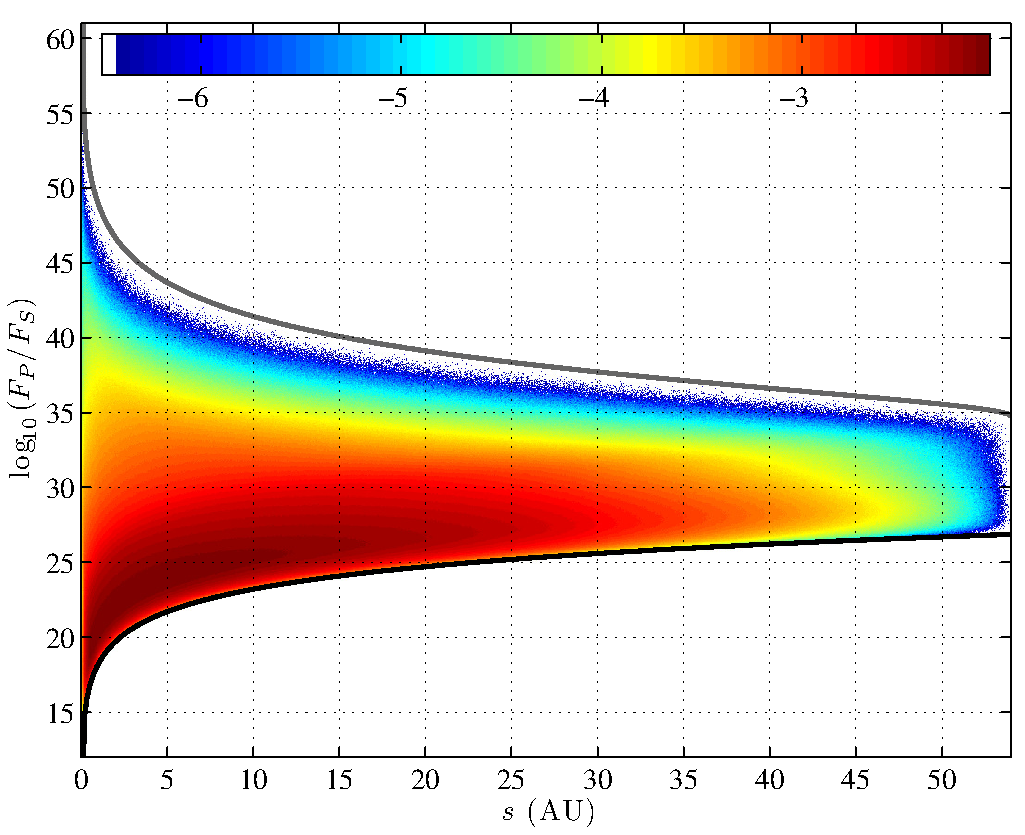
\includegraphics[width=5.5in]{./figures/undersampled_comp_pdf}
 \caption[Undersampled observation PDF]{Observational and photometric completeness for a randomized planetary population  ($a \in [0.4, 30]$, $e \in [0, 0.8]$, $p \in [0.1, 0.5]$, $R \in [0.7, 11.2]R_\oplus$).  The colorbar values and bounding lines are calculated as in \reffig{fig:earthTwin_pdf}. Note that the black line corresponds to high probability areas of the histogram and is thus a good bound, whereas the gray line corresponds to low probability areas and thus demonstrates the undersampling of the Monte Carlo procedure.}
\label{fig:undersampled_comp_pdf} 
\end{figure} 

Any alternate method of sampling the completeness functions introduced in \S\ref{sec:completeness} requires at least some knowledge of their density functions.  In particular, Markov chain methods such as Metropolis-Hastings \citep{hastings1970monte} perform significantly better if the proposal distribution (a function used to `propose' new samples that are then either accepted or rejected) closely approximates the target distribution.  A special case of Metropolis-Hastings, known as Gibbs sampling, can be used to generate a sequence of samples from the joint distribution of two variables if their conditional probabilities are known.  Our goal is to derive the distribution functions of the arguments to the completeness functions.

Following \citet{savransky2011parameter}, we start with an ensemble of Keplerian orbits whose orientation is uniformly distributed in space and derive the distribution functions of these orbits' Keplerian parameters. We make no \emph{a priori} assumptions as to the distribution of orbital semi-major axis and eccentricity, treating them instead as arbitrary functions.  This allows us to derive the completely general distribution functions presented in \S\ref{sec:analytic_dists_deriv}.  A key step here is the demonstration that the planetary phase angle ($\beta$) is independent of any of the orbital parameters.  This makes it possible to write distribution functions for quantities directly related to the two parameters of the direct detection completeness function.  It is important to note that, while the specific application explored here is direct imaging, these distributions are more broadly applicable to exoplanet studies in general.  For example, Keplerian fits are often employed in doppler spectroscopy surveys, making these derivations useful for inferring the true distributions of orbital parameters derived from radial velocity data sets.  Similarly, statistical analyses play an important role in other methods of exoplanet study, including transit photometry and microlensing surveys \citep{gould2010frequency}.

\subsection{Derivation}\label{sec:analytic_dists_deriv}
The distributions of the orbit orienting Euler angles (see \refeq{eq:rpsrot}) are fixed by our assumption of uniform orbital orientation in space.  The remaining two parameters, $a$ and $e$, will be treated as unknowns, with probability density functions (PDFs) $f_{\bar{e}}(e)$ and $f_{\bar{a}}(a)$, respectively. Let $\bar{M}, \bar{e}$ and $\bar{\nu}$ be random variables with the distributions of mean anomaly, eccentricity and true anomaly, respectively, and define two functions: $\nu = g(M,e)$ and $M = h(\nu,e)$.  Following \citet{larson}, we can write the CDF for $\bar{\nu}$ as a marginalization of a conditional probability,
\begin{align} 
F_{\bar{\nu}}(\nu) &= P\left[g(\bar{M},\bar{e}) \le \nu\right] = \int_{-\infty}^{\infty} P\left[g(\bar{M},e) \le \nu | \bar{e} = e\right]f_{\bar{e}}(e)\, \mathrm{d}e\nonumber\\
&=  \int_{0}^{1} P\left[\bar{M} \le h(\nu,e)\right]f_{\bar{e}}(e)\, \mathrm{d}e\,,
\end{align}
where the last step assumes independence between  $\bar{M}$ and $\bar{e}$, and that the orbits are closed so that $e \in [0,1)$.  We note that:
\begin{equation}\label{eq:Mprob}
P[\bar{M} \le h(\nu,e)] = \int_0^{h(\nu,e)} f_{\bar{M}}(M)\, \mathrm{d}M
\end{equation}
where $f_{\bar{M}}(M)$ is the PDF of $M$:
\begin{equation}\label{eq:Mdist}
f_{\bar M}(M) = \left\{
    \begin{array}{l l}
    \frac{1}{2 \pi} & M \; \in \; [0, 2\pi) \\
    0 & \mathrm{else}
    \end{array} \right. \,.
\end{equation}
Therefore the PDF of $\nu$ is:
\begin{equation}\label{eq:nupdf}
f_{\bar{\nu}}(\nu) =  \frac{\mathrm{d}}{\mathrm{d}\nu}F_{\bar{\nu}}(\nu) =  \frac{1}{2\pi} \int_{0}^{1} \frac{\partial h}{\partial \nu}f_{\bar{e}}(e)\, \mathrm{d}e  =  \frac{1}{2\pi} \int_{0}^{1} \frac{\left(1-e^2\right)^\frac{3}{2}}{\left(1+e\cos\nu\right)^2} f_{\bar{e}}(e)\, \mathrm{d}e \, ,
\end{equation}
where $h$ is given by equations (\ref{eq:nutoE}) and (\ref{eq:EtoM}).

Following the same procedure, but without substituting equation (\ref{eq:nutoE}) into equation (\ref{eq:EtoM}), we find that the PDF of the eccentric anomaly is:
\begin{align}
f_{\bar{E}}(E) &=  \int_{0}^{1} \frac{\partial }{\partial E}\left( E - e\sin(E) \right)f_{\bar{M}}(M)f_{\bar{e}}(e)de \nonumber\\
& = \frac{1}{2\pi}\int_{0}^{1} \left(1-e\cos E\right) f_{\bar{e}}(e)\, \mathrm{d}e \,. \label{eq:Edist}
\end{align}
Similarly, if we rewrite the Kepler equation as:
\begin{equation}
M = \cos^{-1}\left(\frac{a - r}{ea}\right) - e\sqrt{1 - \frac{(a-r)^2}{(ea)^2}}
\end{equation}
and assume independence between $\bar a$ and $\bar e$, we can write the PDF for the orbital radius as:
\begin{equation}\label{eq:rpdf}
f_{\bar{r}}(r) = \frac{1}{\pi}\int_{0}^{\infty} \int_{0}^{1} \frac{r}{a\sqrt{(ae)^2 - (a-r)^2}}f_{\bar{e}}(e) \, \mathrm{d}e \, f_{\bar{a}}(a)\, \mathrm{d}a \,.
\end{equation}
Equations (\ref{eq:nupdf}), (\ref{eq:Edist}), and (\ref{eq:rpdf}) are the most complete descriptions possible for the distributions of the orbital position and anomaly, without assuming specific distributions for the eccentricity and semi-major axis.

We derived the distribution functions of the true anomaly and orbital radius by assuming independence between the Keplerian orbital elements from which the anomaly and radius are calculated.  However, the quantities observed by direct searches (i.e., $s$ and $F_R$) are nonlinear functions of the Keplerian elements and $r$, so we cannot make the assumption of independence between their functional arguments for either of these.  Fortunately, inspection of the phase angle reveals something interesting.  Using the approximation in equation (\ref{eq:betadef}), we can write:
\begin{equation}
\beta \approx \cos^{-1}\left(\cos\theta  \cos\nu -\cos\psi  \sin\theta  \sin\nu \right) 
\end{equation}
from which we define a new variable,
\begin{equation} \label{eq:cosBeta}
x \triangleq \cos\beta = \cos\theta  \cos\nu -\cos\psi  \sin\theta  \sin\nu \,.
\end{equation}
If it can be shown that $x$ is uniformly distributed for all distributions of eccentricity, then this would prove that $\beta$ is sinusoidally distributed regardless of the distribution of any other orbital parameter, given only our assumption of uniform orbital orientation.  We do so by considering the characteristic function of $x$,
\begin{equation}
\varphi_{\bar{x}}(t) =  \mathbb{E}\left(e^{i t \bar{x}}\right) = \int_{-\infty}^{\infty} \int_{-\infty}^{\infty} \int_{-\infty}^{\infty} e^{i t x} f_{\bar\nu}(\nu) f_{\bar\psi}(\psi) f_{\bar\theta}(\theta)  \intd{\psi} \intd{\theta} \intd{\nu} \,,
\end{equation}
where $\mathbb{E}$ is the expectation value, and showing that it is equivalent to the characteristic function of a uniformly distributed variable.

The assumption of uniform orbital orientation yields:
\begin{eqnarray}
f_{\bar\psi}(\psi) &=& \left\{
    \begin{array}{l l}
    \frac{1}{2 \pi} & \psi \; \in \; [0, 2\pi) \\
    0 & \mathrm{else}
    \end{array}
    \right. \label{eq:psipdf}\\
f_{\bar\theta}(\theta) &=& \left\{
    \begin{array}{l l}
    \frac{\sin{\theta}}{2} & \theta \; \in \; [0, \pi) \\
    0 & \mathrm{else}
    \end{array}
        \right. \label{eq:thetapdf}
\end{eqnarray}
so that the characteristic function of $x$ becomes:
\begin{equation}
\varphi_{\bar{x}}(t)  = \frac{1}{4 \pi}\int_{-\infty}^{\infty} \int_{0}^{\pi} \int_{0}^{2 \pi}  e^{i t (\cos{\theta}\cos{\nu}- \cos{\psi}\sin{\theta}\sin{\nu})}\intd{\psi} \sin{\theta} \intd{\theta}\, f_{\bar\nu}(\nu) \intd{\nu}
\end{equation}
Performing the integral over $\psi$,
\begin{equation}
    \varphi_{\bar{x}}(t)  = \frac{1}{2}\int_{-\infty}^{\infty} \int_{0}^{\pi}  e^{i t \cos{\theta}\cos{\nu}}  J_{0}\left(t \sin{\theta}\sin{\nu}\right)  \sin{\theta} \intd{\theta}\, f_{\bar\nu}(\nu) \intd{\nu}
\end{equation}
where $J_0$ is the zeroth-order Bessel function of the first kind.
We next perform the integral over $\theta$ using Gegenbauer's finite integral (see equation 12.14(1) in \citet{watson1944treatise}):
\begin{align}
    \int_0^{\pi}  e^{i t \cos{\theta}\cos{\nu}} J_{b-\frac{1}{2}}\left(t \sin{\theta}\sin{\nu}\right) C_a^b{(\cos{\theta})} \sin^{b+\frac{1}{2}}{\theta} \intd{\theta} \nonumber\\
     = \sqrt{\frac{2 \pi}{t}} i^a \sin^{b-\frac{1}{2}}{\nu} \, C_a^b{(\cos{\nu})} J_{a+b}(t)
\end{align}
where $C_a^b$ is a Gegenbauer polynomial.  Choosing $a = 0$ and $b = \frac{1}{2}$ yields $C_a^b(x) = 1$ and the integral becomes:
\begin{equation}
    \int_0^{\pi} e^{i t \cos{\theta}\cos{\nu}} J_{0}\left(t \sin{\theta}\sin{\nu}\right) \sin{\theta} \intd{\theta} = \sqrt{\frac{2 \pi}{t}} J_{\frac{1}{2}}(t)
\end{equation}
Since the half-order Bessel function is defined as:
\begin{equation}
    J_{\frac{1}{2}}(t) = \sqrt{\frac{2}{\pi t}}\sin t
\end{equation}
the characteristic function becomes:
\begin{align}
 \varphi_{\bar{x}}(t)  &= \frac{1}{2} \int_{-\infty}^{\infty} \sqrt{\frac{2 \pi}{t}} \sqrt{\frac{2}{\pi t}}\sin t f_{\bar\nu}(\nu) \intd{\nu} \nonumber\\
&= \frac{\sin t}{t} \int_{-\infty}^{\infty} f_{\bar\nu}(\nu) \intd{\nu} \,.
\end{align}
By definition,
\begin{equation}
\int_{-\infty}^{\infty} f_{\bar\nu}(\nu) \intd{\nu} = 1 \,,
\end{equation}
and thus:
\begin{equation} \label{eq:xChar}
 \varphi_{\bar{x}}(t) = \frac{\sin t}{t} \,.
\end{equation}

If we define a random variable $\bar y \sim U([-1,1])$, its characteristic function will be:
\begin{align}
 \varphi_{\bar{y}}(t) =  \mathbb{E}\left(e^{i t \bar y}\right) &= \int_{-\infty}^{\infty} e^{i t y} f_{\bar y}(y) \intd{y} \nonumber \\
&= \frac{1}{2}\int_{-1}^{1} e^{i t y} \intd{y} = \frac{1}{2}\left(\frac{e^{i t }}{i t} - \frac{e^{-i t }}{i t}\right) \label{eq:uniformChar} \\ 
&= \frac{\sin t}{t} \nonumber \,.
\end{align}
As equations (\ref{eq:xChar}) and (\ref{eq:uniformChar}) are identical, $\bar{x}$ and $\bar{y}$ have the same characteristic function, and thus must have the same underlying distribution.  Since $\bar x$ is uniformly distributed on $[-1, 1]$, $\beta$ is sinusoidally distributed in $[0,\pi)$ for any population of uniformly oriented orbits, independent of the specific distribution of $\bar e$ and $\bar a$.  This finding greatly simplifies our derivation of the distribution functions of the flux ratio and apparent separation.

Returning now to the definition of flux ratio in equation (\ref{eq:fluxRatiodef}), and assuming that we are interested in a particular planet type such that $pR^2$ is approximately constant, we see that the flux ratio is a function of the product of two variables, $m = \Phi(\beta)$ and $n = r^{-2}$.  If we define a random variable $\bar k \triangleq \bar m \bar n$, then it can be shown that:
\begin{equation}\label{eq:distmult}
f_{\bar{k}}(k) = \int_{-\infty}^\infty \frac{1}{n} f_{\bar{m}}\left(\frac{k}{n}\right)f_{\bar{n}}(n)\, \mathrm{d}n
\end{equation}
if $\bar m$ and $\bar n$ are independent \citep{larson}.  As we have demonstrated the independence of $\bar \beta$ from $\bar r$, equation (\ref{eq:distmult}) is applicable.
Using equation (\ref{eq:rpdf}), the CDF of $\bar n$ is given by:
\begin{align}
F_{\bar n}(n) &= P[\bar{r}^{-2} \le n] = P\left[-\frac{1}{\sqrt{n}} \le \bar{r} \le \frac{1}{\sqrt{n}}\right] \nonumber\\
&= \int_{-1/\sqrt{n}}^{1/\sqrt{n}} \frac{1}{2\pi}\int_{0}^{\infty} \int_{0}^{1} \frac{r}{a\sqrt{(ae)^2 - (a-r)^2}}f_{\bar{e}}(e) \, \mathrm{d}e \, f_{\bar{a}}(a)\, \mathrm{d}a \, \mathrm{d}r \\
&= \left. \frac{1}{2\pi}\int_{0}^{\infty} \int_{0}^{1} \sqrt{(ae)^2 - (a-r)^2} + 2 a \tan^{-1}\left(\sqrt{\frac{ae + a - r}{ae - a + r}}\right)\right|_{-1/\sqrt{n}}^{1/\sqrt{n}}\nonumber\\
& \times f_{\bar{e}}(e) \, \mathrm{d}e \, \frac{f_{\bar{a}}(a)}{a}\, \mathrm{d}a \nonumber \,.
\end{align}
The PDF of $n$ is thus:
\begin{align}
f_{\bar n}(n) = \frac{1}{4\pi}\int_{0}^{\infty} \int_{0}^{1}
&n^{-\frac{3}{2}}\left[ \left(C_0 +2a\sqrt{n} - 1\right)^{-\frac{1}{2}} -\left(C_0 - 2a\sqrt{n} - 1\right))^{-\frac{1}{2}}\right] \nonumber\\
& \times f_{\bar{e}}(e) \, \mathrm{d}e \, \frac{f_{\bar{a}}(a)}{a}\, \mathrm{d}a
\end{align}
where $C_0 = a^2(e^2 - 1)n$.  The PDF of $\bar m$ is dependent on the exact form of $\Phi$, but can also be evaluated analytically when $\Phi$ is invertible.  In those cases,
\begin{align}
f_{\bar m}(m) &= f_{\bar \beta}(\Phi^{-1}(m)) \left| \frac{ \mathrm{d}}{ \mathrm{d} m} \Phi^{-1}(m) \right| \label{eq:mpdf}\\
&= 
\left\{
    \begin{array}{c l}
    \frac{1}{2} \sin\left(\Phi^{-1}(m)\right) \left| \frac{ \mathrm{d}}{ \mathrm{d} m} \Phi^{-1}(m) \right|  \quad &  \Phi^{-1}(m) \; \in \; [0, \pi) \\
    0 & \mathrm{else}
    \end{array} \right. \nonumber
\end{align}

This formulation is still problematic when dealing with transcendental functions such as the commonly used phase function of a Lambertian sphere (see \refeq{eq:lambertPhaseFunc}):
\begin{equation}\label{eq:lambertPhase}
\pi \Phi(\beta) = \sin\beta + (\pi - \beta)\cos\beta \, ,
\end{equation}
but, since the domain of the function is restricted to $\beta \in [0,\pi]$, the range of $\Phi$ is single-valued ($\in [1, 0]$), and the function is invertible.  Expanding about $\pi/2$, equation (\ref{eq:lambertPhase}) becomes:
\begin{equation}\label{eq:lambertPhaseSeries}
\Phi(\beta) = \frac{1}{\pi}  + \sum_{k=1}^{\infty} \alpha_k \left(\beta - \frac{\pi}{2}\right)^k \quad\textrm{where}\quad \alpha_k = \frac{d_k}{2 k!}\left(\frac{2 (k-1)}{\pi}\right)^{\frac{d_k + d_{k+1}}{2 d_k}}
\end{equation}
and $d_{1:3} = -1,1,1$, with $d_k = d_{k-1}d_{k-2}d_{k-3}$ for $k > 3$, such that you get the series $d_i = \{-1,1,1,-1,-1,1,1,-1,-1\ldots\}$.  Following \citet{morese1953methods}, we can express the inverse function as the series:
\begin{equation}
\beta = \Phi^{-1}(w) = \frac{\pi}{2}  + \sum_{k=1}^{\infty} b_k \left(w - \frac{1}{\pi}\right)^k 
\end{equation}
where
\begin{equation}
b_k = \frac{1}{k \alpha_1^k} \sum_{x \in X} (-1)^{\vert x \vert} \prod_{r=1}^{\vert x\vert}(k-1+r)  \prod_{i=1}^{k-1}\frac{\left(\alpha_{i+1}/\alpha_1\right)^{x_i}}{x_i!}
\end{equation}
and the space $X$ of sets $x$ is defined as:
\begin{equation}\label{eq:Xspacedef}
X \triangleq \left\{x \in \mathbb{N}^{k-1} : \sum_{i=1}^{k-1} i x_i = k-1\right\} \quad\textrm{with}\quad \vert x\vert \triangleq \sum_i x_i \,.
\end{equation}
The inverse series converges to machine double precision in a finite number of terms, except at the endpoints (0 and 1), which themselves do not need to be computed as they map exactly to $\beta = \pi$ and $\beta = 0$, respectively.

Since $\bar F_R = pR^2 \bar k$, Equations (\ref{eq:distmult}) - (\ref{eq:Xspacedef}) allow us to write:
\begin{align}
f_{\bar F_R}(F_R) = \frac{1}{pR^2}\int_{-\infty}^\infty \frac{f_{\bar{n}}(n)}{n} & \cos\left(\sum_{k=1}^{\infty} b_k \left(\frac{F_R}{npR^2} - \frac{1}{\pi}\right)^k\right)\nonumber\\
&\times \left|\sum_{k=1}^\infty k b_k \left(\frac{F_R}{npR^2} - \frac{1}{\pi}\right)^{k-1} \right| \, \mathrm{d}n \label{eq:FRpdf} \,,
\end{align}
which represents the PDF of the planet-star flux ratio for a population of planets with constant $pR^2$ values (i.e., Earth-twins) modeled as Lambertian reflectors.

While \refeq{eq:FRpdf} is computationally tractable and produces accurate results, the coefficient sets in \refeq{eq:Xspacedef} can be very time consuming to compute when a large number of terms is required for convergence.  This leads us to consider a purely numerical solution that nonetheless produces equally accurate results.  Rather than using series reversion, we can use an iterative numerical method to invert $\Phi(\beta)$ and then calculate the first order derivative of the result via finite differences.  Recalling the definition of $m$, by which $\beta = \Phi^{-1}(m)$, we select an initial value for $\beta$ by fitting and inverting a cubic polynomial to $m = \Phi(\beta)$, resulting in:
\begin{equation}\label{eq:betaCubicEst}
\beta_0 = -5.921m^3+ 9.825m^2 - 6.636m + 2.802
\end{equation}
when $\Phi$ is the Lambert phase function.  Next, we use Newton-Raphson iteration to update the estimate as:
\begin{equation}
\beta_{n+1} = \beta + \frac{1}{\pi - \beta}\left(1 + \frac{\pi - \beta}{\tan\beta}  -  \frac{\pi m}{\sin\beta}\right) \,.
\end{equation}
This function, using the initial estimate in \refeq{eq:betaCubicEst}, converges to machine double precision within 25 iterations for all values of $\beta$, except for the endpoints, which can be simply substituted for their correct values as described above.  By using sufficiently small step sizes, the error produced by estimating the derivative via finite differences can similarly be constrained.

When the number of terms leading to convergence is relatively small (on the order of 50), the space $X$ can be calculated in its entirety.  This is done by first recursively generating all of the unique sets of natural numbers of length $k-1$ that sum to $k-1$.   We generate all of the unique pairs of values that sum to $k-1$, and then recursively augment these sets with all of the sets that sum to the value of the last set element, until no new combinations can be generated.  These sets are encoded as an $N \times k-1$ matrix, where $N$ is the number of unique combinations. For each  entry of this matrix of \emph{value} $i$ (where $i \ne 0$) in the $j$th row, the entry in the $j$th row and $i$th column of a matrix of equivalent size is iterated by one.  The result is a matrix encoding the entire space $X$ in its rows.  This basic process is quite computationally intensive (of order $n^n$), but can be made significantly more efficient by removing redundant sets at every iteration of the recursive set generation, and by employing an efficient sort when filling the final matrix, rather than doing so recursively.  These improvements greatly decrease the computational complexity, bringing the running time down to order $2^n$.  A sample implementation that is capable of generating $X$ for $k-1 = 45$ ($N = 89134$) in under 2 minutes on a single core is presented in \refcode{code:calcRevCoefs}.

Finally, we consider the apparent separation.  The same approximation used in equation (\ref{eq:betadef}) allows us to write:
\begin{equation}
s = r \sin \beta \,.
\end{equation}
If we let $\bar l = \sin\bar\beta$, following equation (\ref{eq:mpdf}):
\begin{equation}\label{eq:lpdf}
f_{\bar l}(l) = f_{\bar \beta}(\sin^{-1}(l)) \left| \frac{ \mathrm{d}}{ \mathrm{d} l} \sin^{-1}(l) \right| = 
\left\{
    \begin{array}{l l}
    \frac{l}{\sqrt{1 - l^2}} & l \; \in \; [0,1) \\
    0 & \mathrm{else} \end{array}\right.
    \end{equation}
Returning to equations  (\ref{eq:rpdf}) and (\ref{eq:distmult}) and now letting $\bar m = \bar r$ and $\bar n = \bar l$, we have:
\begin{equation}\label{eq:spdf}
f_{\bar s}(s) = \frac{1}{\pi}  \int_{0}^1 \int_{0}^{\infty} \int_{0}^{1} \frac{s}{a\sqrt{\left(1 - l^2\right)\left[(ael)^2 - (al-s)^2\right]}}f_{\bar{e}}(e) \, \mathrm{d}e \, f_{\bar{a}}(a)\, \mathrm{d}a \, \mathrm{d}l  \, ,
\end{equation}
which represents the probability density function of the apparent separation.  We now have expressions for the distribution functions of both of the observed quantities of direct imaging planet searches.  While the expressions are quite complex, they are numerically integrable, and can be used to check and improve the efficiency of the sampling of the completeness function.   With an assumed $f_{\bar e}(e)$ and $f_{\bar a}(a)$, equations (\ref{eq:FRpdf}) and (\ref{eq:spdf}), via marginalization and joint sampling, can directly produce the completeness distribution.

\subsection{Validation}
As a check on the derived distribution functions for the true anomaly and orbital radius, we first consider the simplest possible case, where both eccentricity and semi-major axis are uniformly distributed:
\begin{eqnarray}
f_{\bar e}(e) &=& \left\{
    \begin{array}{l l}
   1 & e \; \in \; [0, 1] \\
    0 & \mathrm{else}
    \end{array}
    \right. \label{eq:euniformpdf}\\
f_{\bar a}(a) &=& \left\{
    \begin{array}{l l}
    (a_{max} - a_{min})^{-1} &a \; \in \; [a_{max}, a_{min}] \\
    0 & \mathrm{else}
    \end{array}
        \right. \label{eq:auniformpdf}
\end{eqnarray}
Equation (\ref{eq:nupdf}) then becomes:
\begin{align} \label{eq:nupdfuniform}
f_{\bar{\nu}}(\nu) &=  \frac{1}{2\pi} \int_{0}^{1} \frac{\left(1-e^2\right)^\frac{3}{2}}{\left(1+e\cos\nu\right)^2}\, \mathrm{d}e  \nonumber \\
&= -{}_2F_1(1,2;7/2,\cos^2\nu)\frac{\cos\nu}{5\pi} - \frac{3}{16 \cos^4\nu}\left(4\sin\nu + \cos 2\nu - 3\right)
\end{align}
where ${}_2F_1$ is the Gaussian hypergeometric function:
\begin{equation}\label{eq:gaussHyper}
{}_2F_1(a,b;c;z) = \sum_{k=0}^\infty \frac{(a)_k (b)_k}{(c)_k} \frac{z^k}{k!} \,,
\end{equation}
with the Pochhammer symbol $(\cdot)_k$ defined as:
\begin{align}
(x)_0 &= 1 \,,\\
(x)_k &= \prod_{n=0}^{k-1} (x+n) \,,
\end{align}
and with the value of $c$ limited to the set of natural numbers, i.e., $ c \in  \mathbb{Z}^+ \backslash \left\{0\right\}$.  Equation (\ref{eq:rpdf}) becomes:
\begin{align}
f_{\bar{r}}(r) =\frac{1}{\pi a \left(a_{max} - a_{min}\right)} 
& \left[ 2 r \log\left(\frac{\sqrt{a - r} + \sqrt{r - a}}{\sqrt{2a - r} + \sqrt{r}}\right) \right. \nonumber\\
& {} + a\log\left(a - r\right)+ 2a\log\left(-2\left(r + \sqrt{2ar - r^2}\right)\right)  \label{eq:rpdfuniform}  \\
&  \left.\left.{} + ia\log\left(\frac{32r\left(r - a + i\sqrt{(2a - r)r}\right)}{a}\right) \right]\right|_{a_{min}}^{a_{max}} \nonumber \, .
\end{align}

To check these equations, we generate one million IID samples each from the uniform distributions in Equations (\ref{eq:euniformpdf}), (\ref{eq:auniformpdf}) and (\ref{eq:Mdist}) \citep{press1992numerical}.  From these, we calculate the eccentric anomalies via Newton-Raphson iteration applied to \refeq{eq:EtoM}, and then calculate $\nu$ and $r$ via Equations (\ref{eq:nutoE}) and (\ref{eq:rdef}), respectively (see \S\ref{sec:gen_plan_sys}, Equations (\ref{eq:NewtonRaphson}) - (\ref{eq:E0selection})).  The sample PDFs are calculated  for these two parameters and compared with the results of our closed-form solutions, as shown in Figures \ref{fig:compDistsa} and \ref{fig:compDistsb}.  These plots demonstrate excellent agreement, validating the equations. 

\begin{figure}[ht]
\centering
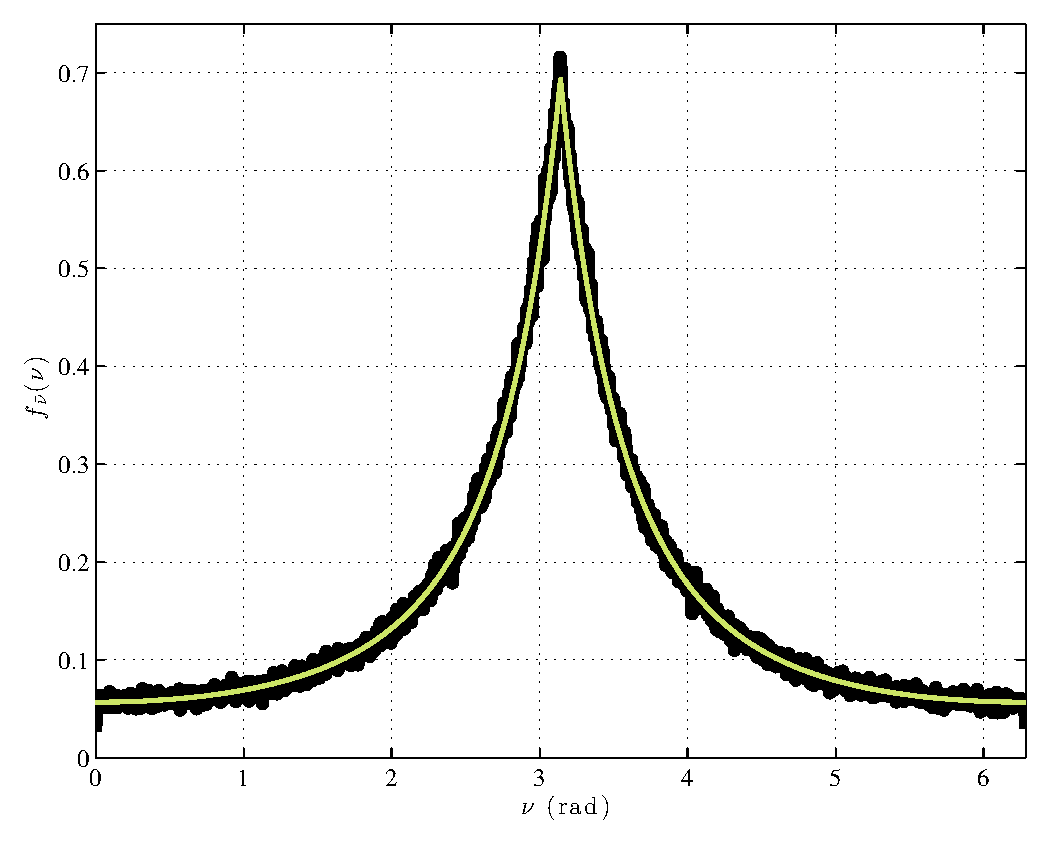
\includegraphics[width=5in]{./figures/compDistsa}
 \caption[Validation of analytical $\nu$ PDF]{ Comparison of empirical (black line) and derived (green line) values of $f_{\bar{\nu}}$ assuming a uniform distribution for $\bar e$. \label{fig:compDistsa}}
\end{figure}  

\begin{figure}[ht]
\centering
\subfigure[$f_{\bar{r}}$, uniform $a$]{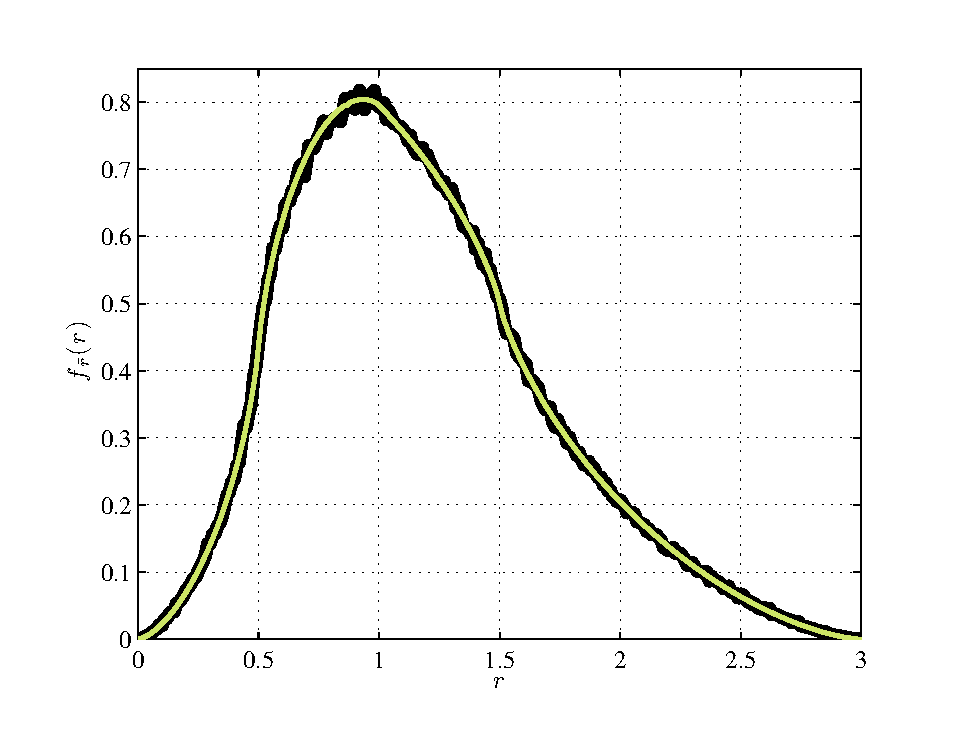
\includegraphics[width=2.95in,clip=true,trim=0.3in 0.1in 0.5in 0.3in]{./figures/compDistsb}\label{fig:compDistsb}}
\subfigure[$f_{\bar{r}}$, log $a$]{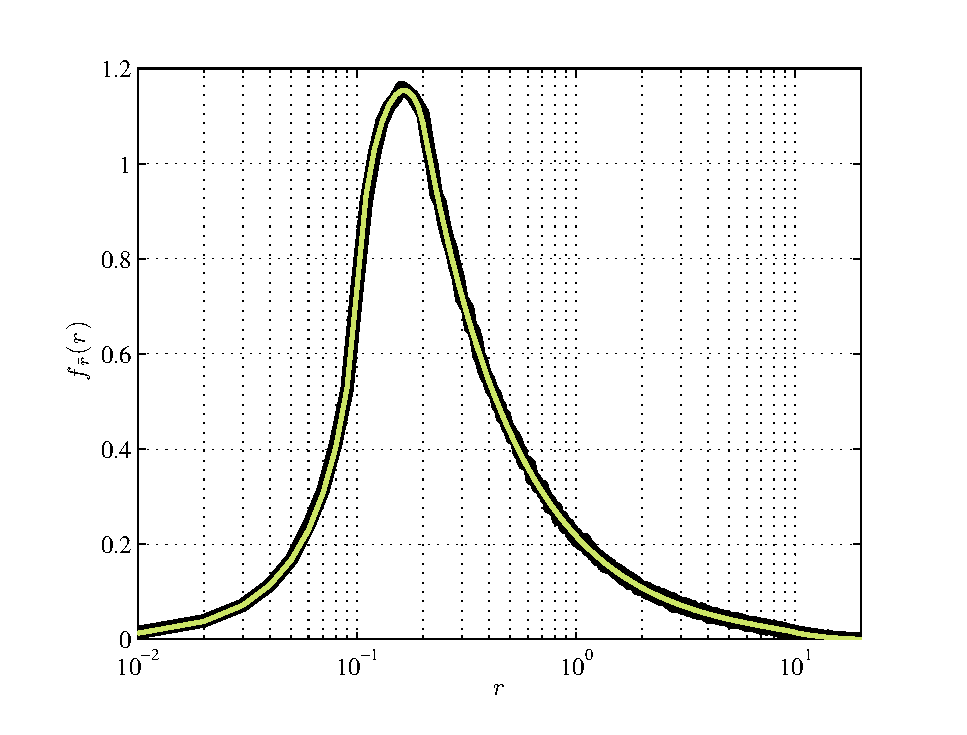
\includegraphics[width=2.95in,clip=true,trim=0.3in 0.1in 0.5in 0.3in]{./figures/compDistsc}\label{fig:compDistsc}}
 \caption[Validation of analytical$r$ PDFs]{ Comparison of empirical (black line) and derived (green line) values for  $f_{\bar{r}}$, assuming a uniform distribution for $\bar e$ and uniform and log distributions for $\bar a$.  For uniformly distributed semi-major axis we have $a \in [0.5, 1.5]$, leading to $r \in (0, 3]$, and for $\bar a$ uniform in $\log a$, we have $a \in [0.1, 10]$ leading to $r \in (0, 20]$. \label{fig:compDists}}
\end{figure}  

While uniform distributions are a useful check, the semi-major axes of currently found planets appear more likely to be logarithmically distributed \citep{currie2009semimajor}. As an additional test, we will assume that $\bar a$ is uniformly distributed in $\log_{10}(a)$ for $a \in [10^{c_{min}}, 10^{c_{max}}]$ so that its PDF is:
\begin{equation}\label{eq:alogpdf}
f_{\bar a}(a) = \left\{
    \begin{array}{l l}
    \left(\Delta c\log(10) a\right)^{-1} &a \; \in \;  [10^{c_{min}}, 10^{c_{max}}]\\
    0 & \mathrm{else}
    \end{array}
        \right.
\end{equation}
where $\Delta c = c_{max} - c_{min}$.
If we retain the same uniform distribution for eccentricity, the true anomaly distribution remains the same, but the orbital radius density becomes:
\begin{align}
f_{\bar{r}}(r) =\frac{1}{2\pi \log(10)\Delta c a^2 r} 
& \left[a\sqrt{(2a - r)r} - a^2\log\left(a - r\right)\right.\nonumber\\
&{} - 2ia^2\log\left(\frac{32 r^3}{a}\left(r - a i \sqrt{(2a - r)r}\right)\right) \nonumber\\
& {} + 2a^2\log\left(-4\left( \sqrt{(2a - r)r^3} + r^2\right)\right)\label{eq:rpdflog}\\
&\left.\left.{} + 2r^2\log\left(\frac{\sqrt{a - r} - \sqrt{r-a}}{\sqrt{2a - r} + \sqrt{r}}\right)\right]\right|_{10^{c_{min}}}^{10^{c_{max}}}\nonumber \, .
\end{align}
We repeat the simulation, this time generating our sample of semi-major axes by exponentiating 10 with a sample of one million uniformly distributed random values between -1 and 1 (thereby setting $\Delta c$ to 2), and re-calculating the PDF for $f_{\bar r}$.  This is compared with the results from \refeq{eq:rpdflog} in \reffig{fig:compDistsc}, and shows excellent agreement.

We can also empirically check the assertion that the distribution of $\beta$ is independent of the distribution of $\bar e$.  We now generate two sets of IID samples, one using the uniform distribution of $\bar e$, and one distributed via a step function,
\begin{equation}\label{eq:piecewise_fe}
f_{\bar e}(e) = \left\{
    \begin{array}{l l}
   1.3 & e \; \in \; [0, 0.7) \\
   0.3 & e \; \in \; [0.7, 1]\\
    0 & \mathrm{else}
    \end{array}
    \right.
\end{equation}
where accurate sampling is achieved via simple rejection sampling.  The two sample sets are used to generate two different sample distributions of $\bar\beta$.  Figure \ref{fig:qqplots} shows Q-Q plots comparing the quantiles of these two samples to the theoretical quantiles of a sinusoidal distribution.  Quantiles for the ideal sinusoidal distribution are calculated by evaluating its inverted CDF at regularly spaced intervals, while quantiles of the two simulated distributions are calculated by ordering and binning the generated values.  As the resulting Q-Q plots follow the 45$^\circ$ line, this demonstrates that the simulated distributions are identical to the theoretical sinusoidal distribution \citep{gibbons2003nonparametric}.
 \begin{figure}[ht]
\centering
\subfigure[Uniform $f_{\bar{e}}$]{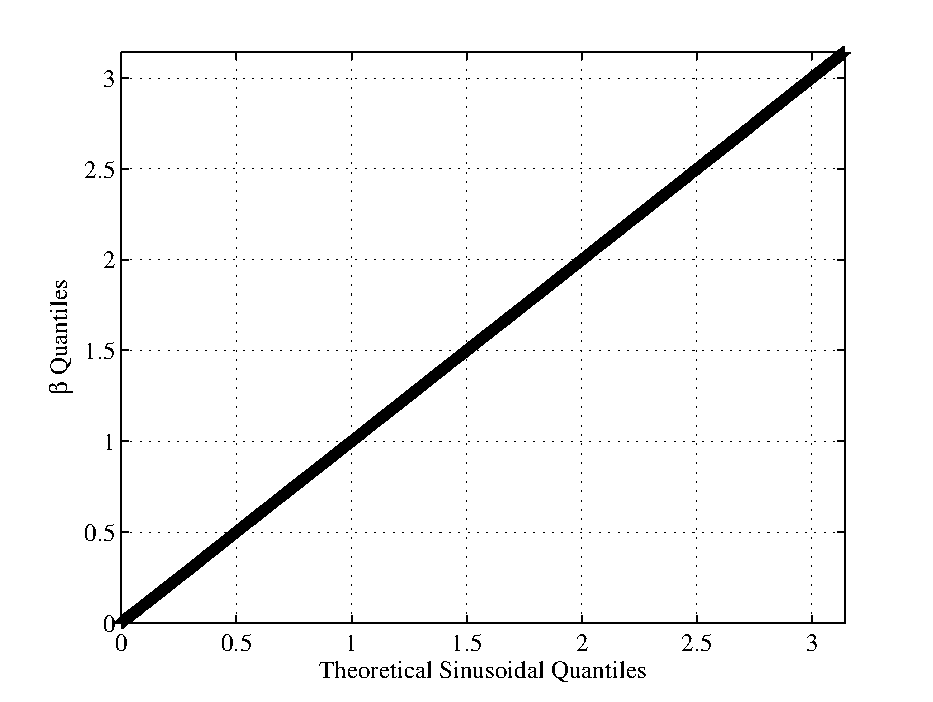
\includegraphics[width=2.95in,clip=true,trim=0.3in 0.1in 0.5in 0.3in]{./figures/qqplota}}
\subfigure[Step $f_{\bar{e}}$]{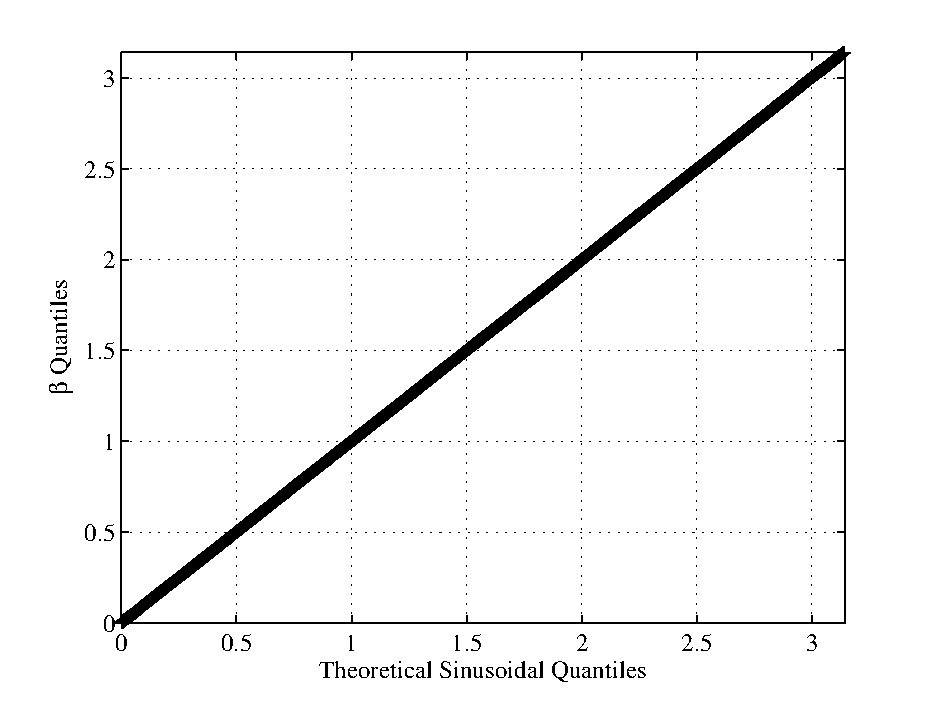
\includegraphics[width=2.95in,clip=true,trim=0.3in 0.1in 0.5in 0.3in]{./figures/qqplotb}}
 \caption[$f_{\bar\beta}$ Q-Q plots]{ Q-Q plots of empirically derived $f_{\bar\beta}$ distributions compared with theoretical sinusoidal quantiles. \label{fig:qqplots}}
\end{figure}

Continuing on to the analytical distributions of the direct detection observables, \refeq{eq:mpdf} allows us to find the PDF of the Lambert Phase function, as shown in \reffig{fig:mdist}.  Similarly, we can use \refeq{eq:spdf} to find the PDF of the apparent separation via quadrature as shown in \reffig{fig:sint}.
\begin{figure}[ht]
\centering
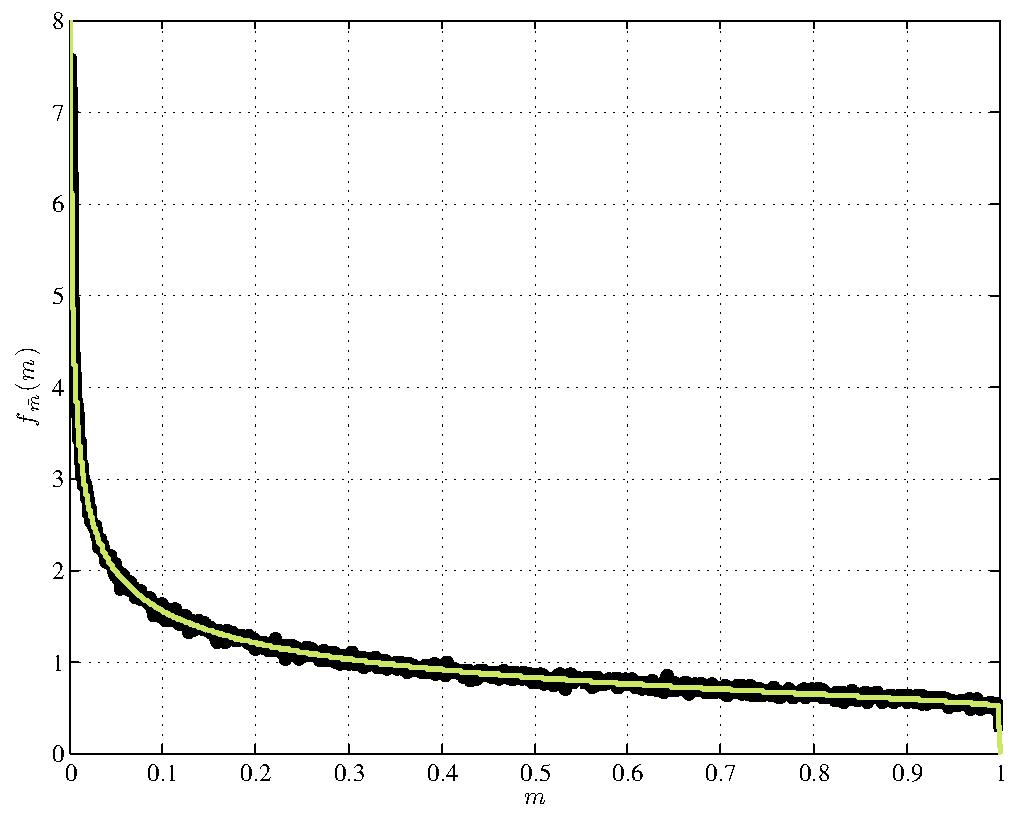
\includegraphics[width=5in]{./figures/mdist}
\caption[Validation of analytical $m$ PDF.]{ Comparison of empirical (black line) and derived (green line) distributions for the Lambert phase function $m = \Phi(\beta)$ for sinusoidally distributed $\beta$. Note that in the derived distribution, the endpoints go to zero and infinity, behavior that is not captured in the empirical distribution. \label{fig:mdist}}
\end{figure}  
\begin{figure}[ht]
\centering
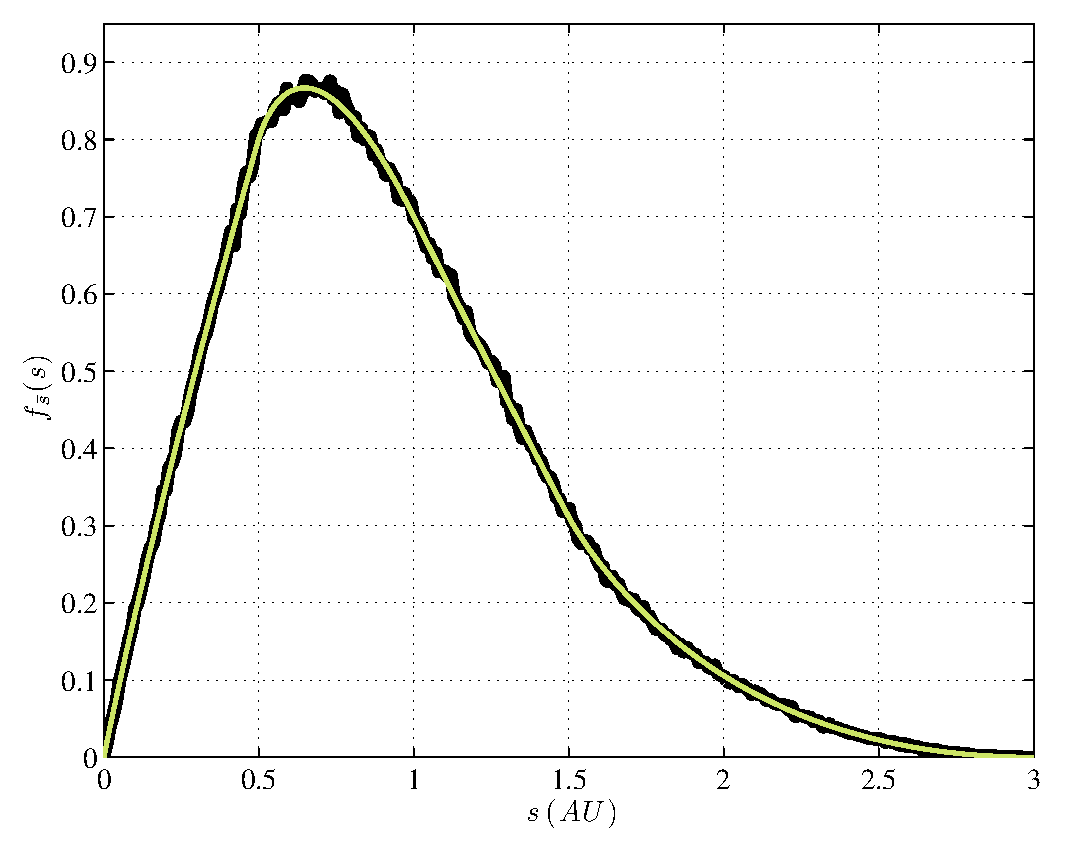
\includegraphics[width=5in]{./figures/sint}
\caption[Validation of analytical $s$ PDF.]{ Comparison of empirical (black line) and derived (green line) distributions assuming the uniform distribution for $\bar e$ and $\bar a$ used in \reffig{fig:compDistsb}. \label{fig:sint}}
\end{figure}

\subsection{Applications}
In addition to improving our ability to sample the completeness function, these analytical distributions have multiple other applications.  One particularly interesting question is how we can use these forms to extract more information from observations and improve overall observing efficiency.  For example, \refeq{eq:spdf} can be used to provide us with information about an orbit's semi-major axis from measurements of apparent separation.  Given a set of measurements of the apparent separation $\left\{s_i\right\}_{i = 1}^n$, the maximum likelihood estimate (MLE) for $a$ is given by \citep{ogunnaike2009random}:
\begin{equation}
\hat a = \arg\max_{a \in \bar a} \hat \ell \left(a \vert s_{1\ldots n}\right)
\end{equation}
where $\hat \ell$ is the likelihood function generally given as:
\begin{equation}
\hat l\left(\theta\vert x_{1\ldots n}\right)= \log f\left(x_{1\ldots n} \vert \theta\right)/n \, .
\end{equation}
Rewriting \refeq{eq:spdf}:
\begin{align}
f_{\bar s}(s) &= \int_a f_{\bar s\vert\bar a}\left(s \vert a\right)f_{\bar{a}}(a)\, \mathrm{d}a\\
& =  \int_{0}^{\infty}\frac{1}{\pi}  \int_{0}^1  \int_{0}^{1} \frac{s}{a\sqrt{\left(1 - l^2\right)\left[(ael)^2 - (al-s)^2\right]}}f_{\bar{e}}(e) \, \mathrm{d}e \, \mathrm{d}l  \,  f_{\bar{a}}(a)\, \mathrm{d}a \nonumber
\end{align}
so that
\begin{equation}
 f_{\bar s\vert\bar a}\left(s \vert a\right)  = \frac{1}{\pi}  \int_{0}^1  \int_{0}^{1} \frac{s}{a\sqrt{\left(1 - l^2\right)\left[(ael)^2 - (al-s)^2\right]}}f_{\bar{e}}(e) \, \mathrm{d}e \, \mathrm{d}l  \,.
\end{equation}
Since the logarithm is a monotonic function, for a single observation of the apparent separation $s = s_0$, the MLE for semi-major axis is therefore:
\begin{equation}\label{eq:aMLE}
\hat a = \arg\max_{a \in \bar a}   \frac{1}{\pi}  \int_{0}^1  \int_{0}^{1} \frac{s_0}{a\sqrt{\left(1 - l^2\right)\left[(ael)^2 - (al-s_0)^2\right]}}f_{\bar{e}}(e) \, \mathrm{d}e \, \mathrm{d}l \,.
\end{equation}

It is clear that the value of $a$ maximizing this equation is equal to $s_0$---i.e., the likeliest value for the semi-major axis given a single observation of the apparent separation is the apparent separation itself, as demonstrated in \reffig{fig:amle}.  Note that the apparent separation can be less than the semi-major axis due to either orientation of the orbit with respect to the line of sight or the orbit's eccentricity.  The apparent separation can be greater than the semi-major axis due only to eccentricity.  As multiple observations of a single exosystem cannot be treated as independent, subsequent measurements of the apparent separation cannot be introduced into the likelihood estimator in \refeq{eq:aMLE}, but may be included in orbital fits.  Nevertheless, the likelihood function can be used to weight each individual observation, and this estimator proves highly useful in the area of mission planning and observation scheduling, as will be discussed in \S\ref{sec:scheduling}.
\begin{figure}[ht]
\centering
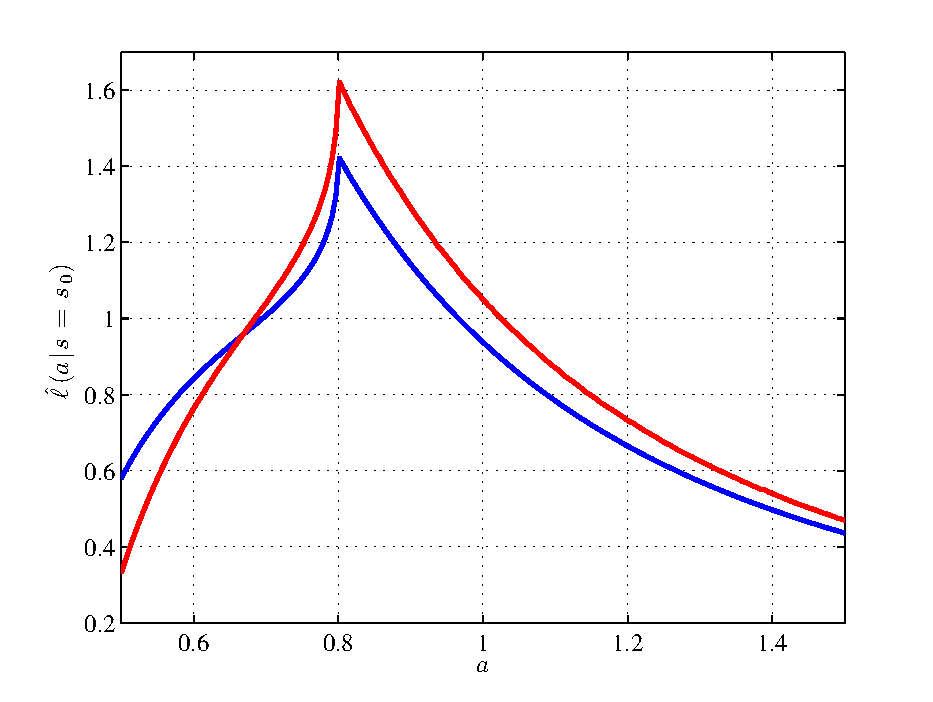
\includegraphics[width=5.5in]{./figures/amle}
\caption[Maximum likelihood for $a$ given $s$.]{Likelihood function for semi-major axis given one observation of apparent separation $s_0 = 0.8$.  $a$ is uniformly distributed $\in [0.5, 1.5]$ and $e$ is distributed either uniformly (blue line) or as in \refeq{eq:piecewise_fe} (red line).  In each case, the value of $a$ maximizing the likelihood function is equal to $s_0$. \label{fig:amle}}
\end{figure}

Returning to the description of transit photometry in \S\ref{sec:photometry}, we see from \refeq{eq:transitFe} that a transit can also be defined in terms of the apparent separation.  In fact, in the simplest possible treatment we can define a generalized transit condition of:
\begin{equation}\label{eq:transitCondition}
s < R_S + R \,.
\end{equation}
Of course, this includes transits that are merely grazing and beyond the sensitivity of available instruments, so the subset of detectable transits is determined by the magnitude of the brightness variation ($F^{(e)}_S/F_S$), just as with direct detections.  However, if we wish to calculate the overall probability of any transit occurring at any point in time, we can simply wirte:
\begin{equation}
P\left[s < R_S + R\right] = \int_0^{R_S + R} f_{\bar s} (s) \intd{s} \,.
\end{equation}
Furthermore, if we consider a particular population of orbits---for example, circular orbits with semi-major axis $a_0$---this further simplifies to:
\begin{equation}
\begin{split}\label{eq:instTransitProb}
P\left[s < R_S + R| a=a_0, e=0\right] &= \int_0^{R_S + R} f_{\bar s} (s) \intd{s} \\
&= \frac{1}{\pi} \int_0^{R_S + R}  \int_{0}^1  \frac{s}{a_0\sqrt{\left(1 - l^2\right)(al-s)^2}} \intd{l} \intd{s}\\
 &= \frac{(R_S + R)^2}{2\pi a_0} \,.
\end{split}
\end{equation}

\begin{figure}[ht]
\centering
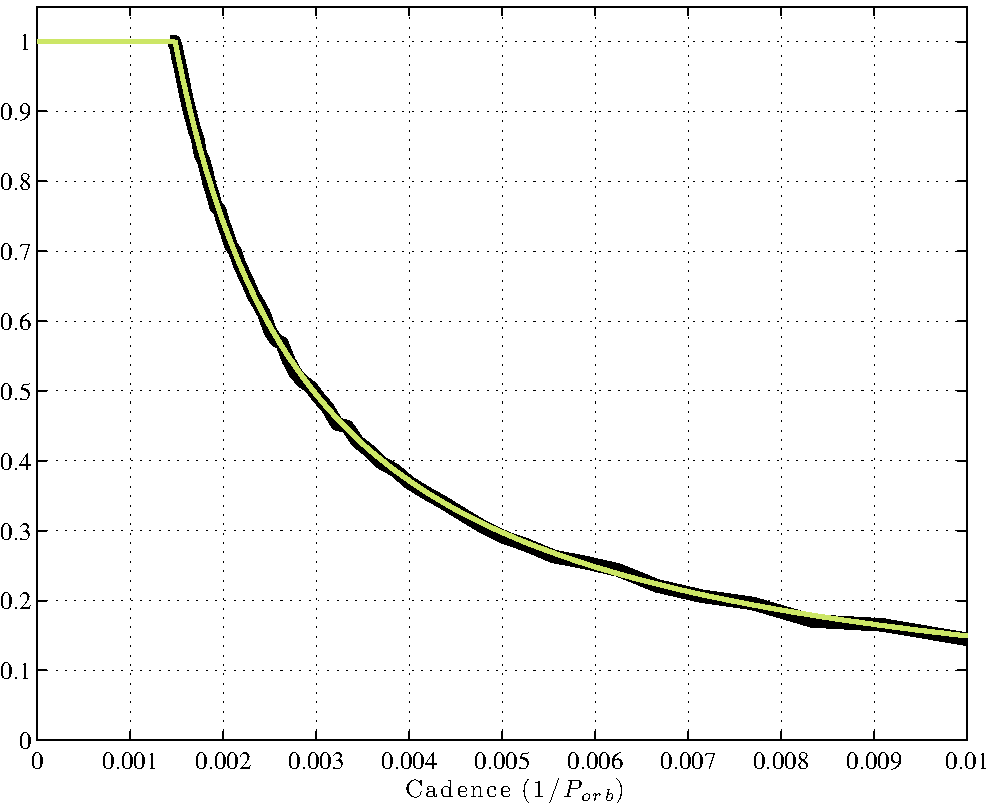
\includegraphics[width=5in]{./figures/transitCadences}
\caption[Portion of observable transits detected over one period.]{Portion of observable transits detected over one orbital period for $a_0 = 1, R_S = R_\odot$ and $R = 0$ as a function of observation cadence. The black line represents the results of simulating one million planets on orbits where transits would occur ($\vert \theta \vert  < R_s/a_0$) and propagating them forward in time by varying time steps.  The green line is defined by \refeq{eq:transitCadenceDropoff}.
\label{fig:transitCadences}}
\end{figure}
While an interesting result, \refeq{eq:instTransitProb} is not very useful on its own, as it represents an instantaneous probability of transits, whereas we are generally interested in the probability of transits over a certain time period (for example, one of the Kepler quarters \citep{borucki2010kepler}).  Every transit photometry survey has a certain cadence of observations as even instruments that monitor stars continuously have a finite integration and readout time.  Therefore, we can model transit observations on a large group of stars as a Poisson process.  While the occurrence of transits about a single star is not independent, if we are merely interested in the portion of monitored stars that will have at least one transit in a given period of time, then we have a collection of random variables representing the number of events occurring throughout a given time interval, each of which is Poisson distributed.  Thus, the portion of target stars with detected transits is a monotonically increasing function in time, with each specific interval having a probability of non-zero transits of:
\begin{equation}
P[N(\Delta t) > 0] = 1 - e^{-\lambda \Delta t} \,
\end{equation}
where $\Delta t$ is the time interval and $\lambda$ is the expected number of occurrences per interval.  This formulation, along with \refeq{eq:instTransitProb}, allows us to calculate the optimal cadence such that 100\% of transits could be captured within one orbital period:
\begin{equation}\label{eq:optimalTransitCadence}
\Delta t_0 = \frac{1}{\pi} \frac{R_s + R}{a_0}
\end{equation}
where this value is in units such that the orbital period associated with $a_0$ (for zero planet mass) is 1.  For any greater time step, the portion of transits discovered within one orbital period is given by:
\begin{equation}\label{eq:transitCadenceDropoff}
\frac{N(\Delta t)}{N(\Delta t_0)} = \frac{\Delta t_0}{\Delta t} + \Delta t \,.
\end{equation}

Of course, the actual portion of transits detected will always be less than unity due to the photometric limitations of the instrument, but the sampling rate in \refeq{eq:optimalTransitCadence} represents the optimal cadence for a given semi-major axis.  Since this interval is inversely proportional to semi-major axis, studies interested in closer-in planets can actually monitor stars fairly infrequently, whereas those looking for further out planets must monitor nearly continuously (as is evident from the geometry of the problem).  \reffig{fig:transitCadences} shows a comparison of  Equations (\ref{eq:optimalTransitCadence}) and (\ref{eq:transitCadenceDropoff}) with results from simulation, demonstrating excellent agreement.

\bigskip
\bigskip

The specific detection method biases, the statistical modeling of exoplanet populations and the concept of completeness are all extremely important to both observation simulation and data analysis.  The next two chapters will demonstrate this using the framework developed here, including the observation timing optimizations.  \refch{ch:obs_sims} will present the details of constructing a planet-finding mission simulation, many of which deal with observation scheduling and are thus greatly informed by completeness and the distributions of planetary parameters. 
